%% Copernicus Publications Manuscript Preparation Template for LaTeX Submissions
\documentclass[gmd, manuscript]{copernicus} %final manuscript
\usepackage{url}
\Urlmuskip=0mu plus 1mu % for better line break in very long globus URLs

%\externaldocument{../PhaseIIPaper/Part1/supdocs/supdoc}

\begin{document}
\title{The GGCMI Phase II experiment: global gridded crop model simulations under uniform changes in CO$_2$, temperature, water, and nitrogen levels (protocol version 1.0)}

\Author[1,2]{James}{Franke}
\Author[3]{Christoph}{M\"{u}ller}
\Author[2,4]{Joshua}{Elliott}
\Author[5]{Alex C.}{Ruane}
\Author[6]{Abigail}{Snyder}
\Author[2,3,4,5]{Jonas}{J\"{a}germeyr}
\Author[7,8]{Juraj}{Balkovic}
\Author[9,10]{Philippe}{Ciais}
\Author[11]{Marie}{Dury}
\Author[12]{Pete}{Falloon}
\Author[7]{Christian}{Folberth}
\Author[11]{Louis}{Fran{\c{c}}ois}
\Author[13]{Tobias}{Hank}
\Author[14,23]{Munir}{Hoffmann}
\Author[15,16]{R.\ Cesar}{Izaurralde}
\Author[11]{Ingrid}{Jacquemin}
\Author[15]{Curtis}{Jones}
\Author[7]{Nikolay}{Khabarov}
\Author[14]{Marian}{Koch}
\Author[2,17]{Michelle}{Li}
\Author[9,18]{Wenfeng}{Liu}
\Author[19]{Stefan}{Olin}
\Author[5,20]{Meridel}{Phillips}
\Author[21,22]{Thomas A.\ M.}{Pugh}
\Author[15]{Ashwan}{Reddy}
\Author[9,10]{Xuhui}{Wang}
\Author[12]{Karina}{Williams}
\Author[13]{Florian}{Zabel}
\Author[1,2]{Elisabeth}{Moyer}
%%%%%%%%%%%%%%%%%%%%%%%%%%%%%%
\affil[1]{Department of the Geophysical Sciences, University of Chicago, Chicago, IL, USA}
\affil[2]{Center for Robust Decision-making on Climate and Energy Policy (RDCEP), University of Chicago, Chicago, IL, USA}
\affil[3]{Potsdam Institute for Climate Impact Research, Member of the Leibniz Association, Potsdam, Germany}
\affil[4]{Department of Computer Science, University of Chicago, Chicago, IL, USA}
\affil[5]{NASA Goddard Institute for Space Studies, New York, NY, United States}
\affil[6]{Joint Global Change Research Institute, Pacific Northwest National Laboratory, College Park, MD, USA}
\affil[7]{Ecosystem Services and Management Program, International Institute for Applied Systems Analysis, Laxenburg, Austria}
\affil[8]{Department of Soil Science, Faculty of Natural Sciences, Comenius University in Bratislava, Bratislava, Slovak Republic}
\affil[9]{Laboratoire des Sciences du Climat et de l'Environnement, CEA-CNRS-UVSQ, 91191 Gif-sur-Yvette, France}
\affil[10]{Sino-French Institute of Earth System Sciences, College of Urban and Env. Sciences, Peking University, Beijing, China}
\affil[11]{Unit{\'{e}} de Mod{\'{e}}lisation du Climat et des Cycles Biog\'eochimiques, UR SPHERES, Institut d'Astrophysique et de G\'eophysique, University of Li\`ege, Belgium}
\affil[12]{Met Office Hadley Centre, Exeter, United Kingdom}
\affil[13]{Department of Geography, Ludwig-Maximilians-Universit\"{a}t, Munich, Germany}
\affil[14]{Georg-August-University G\"{o}ttingen, Tropical Plant Production and Agricultural Systems Modeling, G\"{o}ttingen, Germany}
\affil[15]{Department of Geographical Sciences, University of Maryland, College Park, MD, USA}
\affil[16]{Texas Agrilife Research and Extension, Texas A\&M University, Temple, TX, USA}
\affil[17]{Department of Statistics, University of Chicago, Chicago, IL, USA}
\affil[18]{EAWAG, Swiss Federal Institute of Aquatic Science and Technology, D\"{u}bendorf, Switzerland}
\affil[19]{Department of Physical Geography and Ecosystem Science, Lund University, Lund, Sweden}
\affil[20]{Earth Institute Center for Climate Systems Research, Columbia University, New York, NY, USA}
\affil[21]{School of Geography, Earth and Environmental Sciences, University of Birmingham, Birmingham, UK.}
\affil[22]{Birmingham Institute of Forest Research, University of Birmingham, Birmingham, UK.}
\affil[23]{Leibniz Centre for Agricultural Landscape Research (ZALF), D-15374 Müncheberg, Germany}
%%%%%%%%%%%%%%%%%%%%%%%%%%%%%%
\runningtitle{The GGCMI Phase II experiment: simulating and emulating global crop yield}
\runningauthor{Franke et al.}
\correspondence{Christoph M\"{u}ller (cmueller@pik-potsdam.de)}
%%%%%%%%%%%%%%%%%%%%%%%%%%%%%%
%% These dates will be inserted by Copernicus Publications during the typesetting process.
\received{}
\pubdiscuss{} %% only important for two-stage journals
\revised{}
\accepted{}
\published{}
%%%%%%%%%%%%%%%%%%%%%%%%%%%%%%
\firstpage{1}
\maketitle
%%%%%%%%%%%%%%%%%%%%%%%%%%%%%%
\begin{abstract}
Concerns about food security under climate change motivate efforts to better understand future changes in crop yields.  
Process-based crop models, which represent plant physiological processes, are necessary tools for this purpose since they allow representing future climate and management conditions not sampled in the historical record and new locations to which cultivation may shift. 
However, process-based crop models  differ in many critical details, and their responses to different interacting factors remain only poorly understood. 
The Global Gridded Crop Model Intercomparison (GGCMI) Phase II experiment, an activity of the Agricultural Model Intercomparison and Improvement Project (AgMIP), is designed to provide a systematic parameter sweep across critical interacting factors, to allow both evaluating model behavior and emulating model responses in impact assessment tools.
In this paper we describe the GGCMI Phase II experimental protocol and its simulation data archive. 
Twelve crop models simulate five crops in simulations with systematic uniform perturbations of historical climate, varying CO$_2$, temperature, precipitation, and applied nitrogen (``CTWN'') for rainfed and irrigated agriculture, and a second set of simulations represents adaptation by allowing adjusted planting dates.
We show some crop yield results to illustrate general characteristics of the simulations and potential uses of the GGCMI Phase II archive. 
For example, modeled yields show robust decreases to warmer temperatures in almost all regions, with a nonlinear dependence that means yields in warmer baseline locations have greater temperature sensitivity. 
Inter-model uncertainty is qualitatively similar across all the four input dimensions, but is largest in high-latitude regions where crops may be grown in the future.
\end{abstract}

%\copyrightstatement{TEXT}

\introduction
\label{S:1}
Understanding crop yield response to a changing climate is critically important, especially as the global food production system will face pressure from increased demand over the next century \citep{Foley2005,bodirsky2015}. 
Climate-related reductions in supply could therefore have severe socioeconomic consequences \citep[e.g.][]{Stevanovic2016,Wiebe_2015}. 
Multiple studies using different crop or climate models concur in projecting sharp yield reductions on currently cultivated cropland under {business-as-usual} climate scenarios, although their yield projections show considerable spread \citep[e.g.][and references therein]{Rosenzweig2014, Schauberger2017, porter2014}. 
Although forecasts of future yields reductions can be made with simple statistical models based on regressions in historical weather data, process-based models, which simulate the process of photosynthesis and the biology and phenology of individual crops, play a critical role in assessing the impacts of climate change.

Process-based models are necessary for understanding crop yields in novel conditions not included in historical data, including higher CO$_2$ levels, out-of-sample combinations of rainfall and temperature, cultivation in areas where crops are not currently grown, and differing management practices \citep[e.g.][]{pugh_climate_2016, Roberts2017,minoli2019modelling}. Process-based models have therefore been widely used in studies on future food security \citep{wheeler2013climate, Elliott14, frieler2017assessing}, options for climate mitigation \citep{muller2015} and adaptation \citep{challinor2018improving}, and future sustainable development \citep{humpenoder2018large, jagermeyr_reconciling_2017}.
Process-based models also allow for the globally gridded simulations needed for understanding the global dynamics of agricultural trade, including cultivation area changes and crop selection switching under climate change \citep{rosenzweig2018,ruane2018} because global market mechanisms may strongly modulate climate change impacts \citep{Stevanovic2016,hasegawa2018risk}. 
Global crop model experiments are needed for systematic climate change assessments \citep{muller_global_2017}.

Modeling crop responses continues however to be challenging, as crop growth is a function of complex interactions between climate inputs and management practices \citep{Boote13,rotter2011}. 
Models tend to agree broadly in major response patterns, including a reasonable representation of the spatial pattern in historical yields of major crops and projections of shifts in yield under future climate scenarios \citep[e.g.][]{Elliott2015, muller_global_2017}. 
But process-based models still struggle with some important details, including reproducing historical year-to-year variability in many regions \citep[e.g.][]{muller_global_2017, Jag2018}, reproducing historical yields when driven by reanalysis weather \citep[e.g.][]{Glotter14}, and low sensitivity to extreme events \citep[e.g.][]{Glotter15,schewe2019}. 
Long-term projections therefore retain considerable uncertainty \citep{WOLF2002217, JAGTAP200273, Iizumi2010, ANGULO201332, Asseng2013, Asseng2015}. 

Model intercomparison projects such as the Agricultural Model Intercomparison and Improvement Project \citep[AgMIP, ][]{ROSENZWEIG2013} are crucial in quantifying uncertainties in model projections \citep{Rosenzweig2014}. Intercomparison projects have also been used to develop protocols for evaluating overall model performance \citep{Elliott2015, muller_global_2017} and to assess the representation of individual physical mechanisms such as water stress and CO$_2$ fertilization \citep[e.g.][]{Schauberger2017}.
However, to date, few such projects have systematically sampled critical factors that may interact strongly in affecting crop yields. A number of modeling exercises in the last five years have begun to use
systematic parameter sweeps in crop model evaluation and emulation  \citep[e.g.][]{ruane2014, Markowski2015, Pirttioja2015,FRONZEK20182, Snyder2018, RUIZRAMOS2018}, but all involve limited sites and most also limited crops and scenarios. 

The Global Gridded Crop Model Intercomparison (GGCMI) Phase II experiment is the first globally gridded crop model intercomparison involving a systematic parameter sweep across critical interacting factors.
GGCMI Phase II is an activity of the Agricultural Model Intercomparison and Improvement Project (AgMIP), 
and a continuation of a multi-model comparison exercise begun in 2014. 
The initial GGCMI Phase I compared harmonized yield simulations over the historical period, with primary goals of model evaluation and understanding sources of uncertainty (including model parameterization, weather inputs, and cultivation areas) \citep{Elliott2015, muller_global_2017, folberth2016, porwollik_spatial_2016}. 
GGCMI Phase II compares simulations across a set of inputs with uniform perturbations to historical climatology,  
including CO$_2$, temperature, precipitation, and applied nitrogen (collectively referred to as ``CTWN''), as well as adaptation to shifting growing seasons. 
The CTWN experiment is inspired by AgMIP's Coordinated Climate-Crop Modeling Project \citep[C3MP][]{ruane2014,mcdermid2015agmip} and contributes to the AgMIP Coordinated Global and Regional Assessments (CGRA) \citep{ruane2018, rosenzweig2018}. 

In this paper, we describe the GGCMI Phase II model experiments and present initial summary results.
In the sections that follow, we describe the experimental goals and protocols; the different process-based models included in the intercomparison; the levels of participation by the individual models. We then provide an assessment of model fidelity based on observed yields at the country level, and show some selected examples of the simulation output dataset to illustrate model responses across the input dimensions.

%%%%%%%%%%%%%%%%%%%%%%%%%%%%%%%%%%%%%%%%%%%%%%%%%%%%%%%%%%%%%%%s
%%%%%%%%%%%%%%%%%%%%%%%%%%%%%%%%%%%%%%%%%%%%%%%%%%%%%%%%%%%%%%%
%%%%%%%%%%%%%%%%%%%%%%%%%%%%%%%%%%%%%%%%%%%%%%%%%%%%%%%%%%%%%%%
\section{Simulation objectives and protocol}
\label{S:2}
\subsection{Goals}

The guiding scientific rationale of GGCMI Phase II is to provide a comprehensive, systematic evaluation of the response of process-based crop models to critical interacting factors, including CO$_2$, temperature, water, and applied nitrogen (CTWN). 
The dataset is designed to allow researchers to:
\begin{itemize}
    \item Enhance understanding of models’ sensitivity to climate and nitrogen drivers.
    \item Study the interactions between climate variables and nitrogen inputs in driving modeled yield impacts. 
    \item Characterize differences in crop responses to climate change across the Earth's climate regions.
    \item Provide a dataset that allows statistical emulation of crop model responses for downstream modelers.
    \item Explore the potential effects on future yield changes of adaptations in growing season length.
\end{itemize}
\vspace{-0.05in}

\subsection{Modeling protocol}
\begin{figure*}[ht]
  \centering
  \includegraphics[width=15cm]{figures/number_of_models.png}
  \caption{
  \textbf{Left panel:}Cultivated areas for maize, rice, and soybean are taken from the MIRCA2000 (``Monthly Irrigated and Rainfed Crop Areas around the year 2000'') dataset \citep{Portmann2010}. 
  Areas for winter and spring wheat areas are adapted from MIRCA2000 and two other sources; see text for details.  For irrigated crops, see supplemental Figure S1.
  \textbf{Right panel:} Number of models providing simulations for each grid cell.  
  All models provide the minimum areal coverage of the GGCMI Phase II protocol, but some provide extra coverage at high latitudes or in arid or otherwise unsuitable areas.}
  \label{fig:crop_area}
\end{figure*}

The GGCMI Phase I intercomparison was a relatively limited computational exercise, requiring yield simulations for 19 crops across a total of 310 model-years of historical scenarios, and had the participation of 21 modeling groups.
The GGCMI Phase II protocol is substantially larger, involving over 1400 individual 30-year scenarios, or over 42,000 model-years; 12 modeling groups nevertheless participated. To reduce the computational load, the GGCMI Phase II protocol reduces the number crops to 5 (maize, rice, soybean, spring wheat, and winter wheat). 
The reduced set of crops includes the three major global cereals and the major legume and accounts for over 50\% of human calories in 2016: nearly 3.5 billion tons or 32\% of total global crop production by weight \citep{FAOSTAT}. 
This set of major crops has the advantage of historical yield data globally available at sub-national scale \citep{Ray2012,iizumi_historical_2014}, and has been frequently used in previous analyses \citep[e.g.][]{muller_global_2017,porwollik_spatial_2016}.

The Phase II protocol involves a suite of uniform perturbations from a historical climate timeseries.
The baseline climate scenario for GGCMI Phase II is one of the weather products used in Phase I, daily climate inputs for 1980-2010 from the 0.5 degree NASA AgMERRA (``Agricultural''-modified Modern Era Retrospective analysis for Research and Applications) gridded re-analysis product. AgMERRA is specifically designed for agricultural modeling, with satellite-corrected precipitation \citep{Ruane2015}. 
The experimental protocol consists of 9 levels for precipitation perturbations, 7 for temperature, 4 for CO$_2$, and 3 for applied nitrogen, for a total of 756 simulations, 672 for rainfed agriculture and an additional 84 for irrigated (Table \ref{table:inputs}). 
%For irrigated simulations, models are set to apply near-perfect irrigation to keeps soils wet throughout the entire growing period, with no limitations in water supply. 
In irrigated simulations, crops are assumed to have no water constraints, i.e. all crop water requirements are fulfilled regardless of local water supply limitations.
Values of climate variable perturbations are selected to represent reasonable ranges for changes over the medium term (to 2100) under business-as-usual emissions. 
The resulting GGCMI Phase II dataset therefore captures the distribution of crop model responses over the range of potential future climate conditions.

\begin{table}[t]
  \caption{
  GGCMI Phase II input parameter levels for each dimension. Temperature and precipitation values indicate the perturbations from the historical climatology. Irrigated (W$_{inf}$) simulations assume the maximum beneficial levels of water Bold font indicates the `baseline' or historical level for each dimension. One model provided simulations at the T + 5 level.
  }
  \label{table:inputs} 
  \begin{tabular}{lcc} 
      \tophline \vspace{1mm}
      \textbf{Input variable} & \textbf{Simulation input values} & \textbf{Unit} \\ \middlehline \vspace{1mm}
      CO$_2$ (C) & \textbf{360}, 510, 660, 810 & ppm\\ \middlehline \vspace{1mm}
      Temperature (T) & -1, \textbf{0}, 1, 2, 3, 4, 6 & $^{\circ}$C\\ \middlehline \vspace{1mm}
      Precipitation (W) & -50, -30, -20, -10, \textbf{0}, & \% \\
      {} & 10, 20, 30, (and W$_{inf}$) & {} \\ \middlehline \vspace{1mm}
      Applied nitrogen (N) & 10, 60, \textbf{200} & kg ha$^{-1}$ \\ \middlehline \vspace{1mm}
      Adaptation (A) & \textbf{A0: none}, A1: new cultivar to maintain original growing season length & -\\ \bottomhline
  \end{tabular}\\
\end{table}

While all perturbations are applied uniformly across the historical timeseries, they are applied in different ways. 
While precipitation perturbations are applied as fractional changes, temperature perturbations are applied as absolute offsets from the daily mean, minimum, and maximum temperature timeseries for each grid cell.
CO$_2$ and nitrogen levels are specified as discrete values applied uniformly over all grid cells. 
The protocol samples over all possible permutations of individual perturbations.
This choice means that CO$_2$ changes are applied independently of changes in climate variables, so that higher CO$_2$ is not associated with particular climate changes, e.g.\ higher temperatures. 

Each model is run at 0.5 degree spatial resolution and covers all currently cultivated areas and much of the uncultivated land area. 
Figure \ref{fig:crop_area}, left, shows the present-day cultivated area of rainfed crops and Supplemental Figure S1 that for irrigated crops. 
Cultivated areas are provided by the MIRCA2000 (Monthly Irrigated and Rainfed Crop Area) data product \citep{Portmann2010}.
Coverage extends considerably outside currently cultivated areas because cultivation will likely shift under climate change.  
To reduce the computational burden, however, the protocol requires simulation only over 80\% of Earth land surface area.  
Areas are not simulated if they are assumed to remain non-arable even under an extreme climate change; these regions include Greenland, far-northern Canada, Siberia, Antarctica, the Gobi and Sahara Deserts, and Central Australia.
The protocol also eliminates regions judged unsuitable for cropland for non-climatic reasons. 
Selection criterion involve a combination of soil suitability indices at 10 arc-minute resolution and excludes those 0.5 degree grid cells in which at least 90\% of the area is masked as unsuitable according to any single index, and which do not contain any currently cultivated cropland. 
Soil suitability indices measure excess salt, oxygen availability, rooting conditions, toxicities, and workability, and are provided by the IIASA (International Institute for Applied Systems Analysis) Global Agro-Ecological Zone model \citep[GAEZ, ][]{gaez}. 
The procedure follows that proposed by \citet{pugh_climate_2016}. 
All modeling groups simulate the minimum required coverage, but some provide simulations that extend into masked zones, including e.g.\ the Sahara Desert and Central Australia (Figure \ref{fig:crop_area}, right).

\subsection{Harmonization between models}
The 12 models included in GGCMI Phase II are all process-based crop models that are widely used in impacts assessments (Table \ref{table:models}).
Although some models share a common base (e.g.\ the LPJ family or the EPIC family of models), they have subsequently developed independently.  
Wherever possible, the GGCMI Phase II protocol harmonizes inputs, but differences in model structure mean that several key factors cannot be fully standardized across the experiment. 
These include soil treatment (which affects soil organic matter and carry-over effects of soil moisture across growing years) and baseline climate inputs.  

While 10 of the 12 models participating in GGCMI Phase II use the AgMERRA historical daily climate data product, two models require sub-daily input data and thus use different baseline climate inputs:
PROMET uses ERA-Interim reanalysis \citep{dee2011era}; JULES uses a bias-corrected version of ERA-Interim, the 3-hour WFDEI (WATCH-Forcing-Data-ERA-Interim) \citep{weedon2014wfdei}, selecting WFDEI version with precipitation bias-corrected against the CRU TS3.101/TS3.21 precipitation totals \citep{harris_cru_2014}.
The data products show some differences (Figures S3-S4, which compare data products over currently cultivated areas for each crop during their growing seasons). 
For example, for maize, ERA-Interim daily precipitation is biased high from that in AgMERRA by 7\% (< 1 sigma), while mean daily precipitation in WFDEI is only 3\% higher. 
Precipitation differences are largest in wheat areas, where ERA-Interim is substantially wetter (+60mm year$^{-1}$). 
Temperatures for maize are very similar between data products, with ERA-Interim 0.45$^\circ$C cooler and WFDEI 0.1$^\circ$C warmer. 
Differences are largest for rice, with ERA-Interim 1$^\circ$C cooler. 
These differences are relatively small compared to the perturbations tested in the protocol.

Planting dates and growing season lengths are standardized across models, following the procedure described in \citet{Elliott2015} for the \textit{fullharm} setting. 
In contrast to GGCMI Phase I \citep{Elliott2015}, we here assume identical growing seasons for rainfed and irrigated scenarios, to allow for direct comparability of simulations along the W dimension, in which irrigation (W$_{inf}$) is one element. (See Table \ref{table:inputs}.) 
While sowing dates are prescribed directly and held fixed in models, the length of the growing season is a product of crop phenology, which in turn is mostly driven by phenological parameters and temperature. 
Modelers are asked to adjust the phenological parameters so that growing season length on average matches the harmonization target. 
Given that temperature varies between years, individual years can vary from the harmonization target.
Growing seasons are harmonized across models but are crop- and location-specific.
For example, at present maize is sown in March in Spain, in July in Indonesia, and in December in Namibia \citep{Portmann2010}.
The one exception to the harmonization protocol described above involves CARAIB, which for technical reasons kept their own growing season specifications rather than tuning to standard lengths.
 
Because harvest dates are a function of climate parameters, simulations with the harmonized phenological parameters described above generally result in shorter growing seasons in future warmer scenarios. 
We denote these simulations as ``A0'' experiments, where 0 denotes ``no adaptation''. 
To account for potential adaptation in crop cultivars, the GGCMI Phase II protocol includes a second set of experiments, ``A1'', that assume that cultivars are modified to adjust to changes along the T dimension in the CTWN experiment. 
For these simulations, modelers adjust parameters to hold growing season length approximately constant across the different warming scenarios. 
(CARAIB simulations follow the same principle, fixing growing season length at their baseline levels.) 
The A1 simulations roughly capture the case in which adaptive crop cultivar choice ensures that crops reach maturity at roughly the same time as in the current temperature regime. 
This assumption is simplistic, and does not reflect realistic opportunities and limitations to adaptation \citep{vadez2012adaptation,challinor2018improving}, but provides some insight into how crop modifications could alter projected impacts on yields.

Growing seasons for maize, rice, and soybean are taken from the SAGE (Center for Sustainability and the Global Environment, University of Wisconsin) crop calendar \citep{Sacks2010} and are identical to those used in GGCMI Phase I \citep{Elliott2015}.
In GGCMI Phase II, we separately treat spring and winter wheat and so must define different growing seasons for each.
We use the SAGE crop calendar, which separately specifies spring and winter wheat, as the primary source for 69\% of grid cells. 
In the remaining areas where no SAGE information is available, we turn to, in order of preference, the MIRCA2000 crop calendar \citep{Portmann2010} and to simulated LPJmL growing seasons \citep{waha2012climate}.  
These datasets each provide several options for wheat growing season for each grid cell, but do not label them as spring or winter wheat. We assign a growing season to each wheat type for each location based on its baseline climate conditions. 
A growing season is assigned to winter wheat if all of the following hold, and to spring wheat otherwise
:

\begin{itemize}
  \item{the monthly mean temperature is below freezing point (<0$^\circ$C) at most for 5 months per year (i.e. winter is not too long)}
  \item{the coldest 3 months of a year are below 10$^\circ$C (i.e.\ there is a winter)}
  \item{the season start date fits the criteria that:}
  \item[]{\begin{itemize}  
      \item{if in the N.\ hemisphere, it is after the warmest \textit{or} before the coldest month of the year (as winter is around the end/beginning of the calendar year)}
      \item{if in the S.\ hemisphere, it is after the warmest \textit{and} before the coldest month of the year (as winter is in the middle of the calendar year)}
      \end{itemize}}
\end{itemize}

Nitrogen application is standardized in timing across models. 
N fertilizer is applied in two doses, as is often the norm in actual practice, to reduce losses to the environment. 
In the GGCMI Phase II protocol, half of the total fertilizer input is applied at sowing and the other half on day 40 after sowing, for all crops except for winter wheat. 
For winter wheat, in practice the application date for the second N fertilizer application varies according to local temperature, because the length of winter dormancy can vary strongly. 
In the GGCMI Phase II protocol, the second fertilization date for winter wheat must lie at least 40 days after planting and no later than 50 days before maturity.

If those limits permit, the second fertilization is set to the middle day of the first month after sowing that has average temperatures above 5C.

All stresses in models are disabled other than those related to nitrogen, temperature, and water. 
For example, model responses to alkalinity, salinity, and non-nitrogen nutrients are all disabled. 
No other external N inputs are permitted -- that is, there is no atmospheric deposition of nitrogen --  but some models allow additional release of plant-available nitrogen through mineralization in soils. 
Soil mineralization is a part of model treatments of soil organic matter and cannot be disabled in some models (e.g. LPJmL, LPJ-GUESS). 
Some additional differences in model structure mean that several key factors are not standardized across the experiment. 
For example, carry-over effects across growing years including residue management and soil moisture are treated differently across models.

\subsection{Output data products}
All models in GGCMI Phase II provide 7 mandatory output variables if available (Table \ref{table:outputs}, bold).
For each scenario, 0.5 degree grid cell and crop, models provide 30-year timeseries of annual crop yields in units of tons ha$^{-1}$ year$^{-1}$, as well as total aboveground biomass yield; the dates of planting, anthesis, and maturity; applied irrigation water in irrigated scenarios; and total evapotranspirtation. 
(Note that several of the EPIC-family models do not output the anthesis date.)
Besides these mandatory 7 data products, the protocol requests any or all of 18 optional additional output variables (Table \ref{table:outputs}, plain text).
Participating modeling groups provided between 3 (PEPIC) and 18 (APSIM-UGOE) of these optional variables. 

\begin{table}[]
  \caption{Output variables, naming convention, and units in the GGCMI Phase II protocol. Items in \textbf{bold} are the mandatory minimum requirements. Other variables are optionally provided depending on availability and participating modeling groups provided between 3 (PEPIC) and 18 (APSIM-UGOE) of these optional variables.}
  \label{table:outputs}
  \begin{tabular}{lll}
    \tophline \vspace{1mm}
    Variable                                & variable name             & units \\
    \middlehline \vspace{1mm}
    \textbf{Yield}                                   & \textbf{yield\_<crop>}     & \textbf{t ha$^{-1}$ yr$^{-1}$ (dry matter)}\\
    \textbf{Total above ground biomass yield}        & \textbf{biom\_<crop>}      & \textbf{t ha$^{-1}$ yr$^{-1}$ (dry matter)}\\
    \textbf{Actual planting date}                    & \textbf{plant-day\_<crop>} & \textbf{day of year}\\
    \textbf{Anthesis date}                           & \textbf{anth-day\_<crop>}  & \textbf{days from planting} \\
    \textbf{Maturity date}                           & \textbf{maty-day\_<crop>}  & \textbf{days from planting}\\
    \textbf{Applied irrigation water}                & \textbf{pirrww\_<crop>}    & \textbf{mm yr$^{-1}$} \\
    \textbf{Evapotranspiration (growing season sum)} & \textbf{etransp\_<crop>}   & \textbf{mm yr$^{-1}$ (firr scenarios only)}\\ \middlehline
    Transpiration (growing season sum)                       & transp\_<crop>    & mm yr$^{-1}$ \\
    Evaporation (growing season sum)                         & evap\_<crop>      & mm yr$^{-1}$ \\
    Runoff (total growing season sum, subsurface + surface)  & runoff\_<crop>    & mm yr$^{-1}$                    \\
    Total available soil moisture in root zone *             & trzpah2o\_<crop>  & mm yr$^{-1}$                    \\
    Total root biomass                                       & rootm\_<crop>     & t ha$^{-1}$ yr$^{-1}$ (dry matter)  \\
    Total Reactive Nitrogen (Nr) uptake (growing season sum) & tnrup\_<crop>     & kg ha$^{-1}$ yr$^{-1}$              \\
    Total Nr inputs (growing season sum)                     & tnrin\_<crop>     & kg ha$^{-1}$ yr$^{-1}$              \\
    Total Nr losses (growing season sum)                     & tnrloss\_<crop>   & kg ha$^{-1}$ yr$^{-1}$              \\
    Gross primary production (GPP)                           & gpp\_<crop>       & gC m$^{-2}$ yr$^{-1}$               \\
    Net primary production (NPP)                             & npp\_<crop>       & gC m$^{-2}$ yr$^{-1}$               \\
    CO$_2$ response scaler on NPP                            & co2npp\_<crop>    & - \{0..inf\}                \\
    Water response scaler on NPP                             & h2onpp\_<crop>    & - \{0..1\}                  \\
    Temperature response scaler on NPP                       & tnpp\_<crop>      & - \{0..1\}                  \\
    Nr response scaler on NPP                                & nrnpp\_<crop>     & - \{0..1\}                  \\
    Other nutrient response scaler on NPP                    & ornpp\_<crop>     & - \{0..1\}                  \\
    CO$_2$ response scaler on transpiration                  & co2trans\_<crop>  & - \{0..1\}                  \\
    Maximum stress response scaler                           & maxstress\_<crop> & - \{0..1\}                  \\
    Maximum Leaf Area Index (LAI)                            & laimax\_<crop>    & m$^{2}$ m$^{-2}$           \\        
    \bottomhline
    * growing season sum, basis for computing average soil moisture & {} & {} \\
  \end{tabular}
\end{table}

All output data is supplied as netCDF version 4 files, each containing values for one variable in a 30-year timeseries associated with a single scenario, for all grid cells. File names follow the naming conventions of GGCMI Phase I \citep{Elliott2015}, which themselves are taken from those of ISIMIP \citep{frieler2017assessing}. 
File names are specified (in small caps) as 

$[model]\_[climate]\_hist\_fullharm\_[irrig.scenario]\_[variable]\_[crop]\_global\_annual\_[start-year]\_[end-year].nc4$

\noindent Here $[model]$ is the crop model name; $[climate]$ is the original climate input dataset (typically AgMERRA); $[irrig.scenario]$ is the irrigation setting (``firr'' for fully irrigated and ``noirr'' for fully rainfed); $[variable]$ is the output variable (of those in Table \ref{table:outputs}); $[crop]$ is the crop abbreviation (``mai'' for maize, ``ric'' for rice, ``soy'' for soybean, ``swh'' for spring wheat, and ``wwh'' for winter wheat); and $[start-year]$ and $\_[end-year]$ specify the first and last years recorded on file.
All filenames include the identifier $global$ to distinguish them as global model output.

Output data is provided on a regular geographic grid, identical for all models. 
Grid cell centers span latitudes -89.75 to 89.75$^{\circ}$ and longitudes from -179.75 to 179.75$^{\circ}$. 
Missing values  where no crop growth has been simulated are distinguished from crop failures: a crop failure is reported as zero yield but non-simulated areas (including ocean grid cells) have yields reported as 1.e+20. 
Following NetCDF standards, latitude, longitude and time are included as separate variables in ascending order, with
units ``degrees north'', ``degrees east'', and ``growing seasons since 1980-01-01 00:00:00''. 

Following GGCMI Phase I standards, the first entry in each file describes the first complete cropping cycle simulated from the given climate input timeseries. 
In the AgMERRA timeseries used for GGCMI Phase II, the first year provided is 1980 but the date of the first entry can vary by crop and location. 
In the northern hemisphere, for summer crops like maize (sown in Spring 1980 and harvested in Fall 1980), the first harvest record would be of 1980, but for winter wheat (sown in Fall 1980 and harvested in Spring 1981) the first harvest record would be of 1981. Output files report the sequence of growing periods rather than calendar years. 
While there is generally one sowing event per calendar year (since simulations do not permit double-cropping), in some cases harvest events may skip or repeat within a calendar year. For example, because soybeans in North Carolina are typically harvested well into December, some calendar years may include no harvest (if it is not completed until after Dec. 31) or two harvests (one in January and one 11 months later in the following December). 

\section{Models contributing}
\label{S:3}
\begin{table*}[t]
\caption{
Models included in GGCMI Phase II and the number of CTWN simulations performed. 
The maximum number is 756 for A0 (no adaptation) experiments, and 648 for A1 (maintaining growing length) experiments, since T0 is not simulated under A1. ``N-Dim.'' indicates whether the models are able to represent varying nitrogen levels.
Each model provides the same set of CTWN simulations across all its modeled crops, but some models omit individual crops. (For example, APSIM does not simulate winter wheat.)
}
\label{table:models}
  \begin{tabular}{p{6cm} p{1cm} p{1cm} p{1cm} p{1cm} p{1cm} p{1cm} p{1.9cm}}
    \tophline
    {\textbf{Model (Key Citations)}}&{\textbf{Maize}}&{\textbf{Soybean}}&{\textbf{Rice}}&{\textbf{Winter wheat}}&{\textbf{Spring wheat}}&{\textbf{N dim.}}&{\textbf{Sims per crop (A0 / A1)}}\\ \middlehline
    {\textbf{APSIM-UGOE},   \citet{KEATING2003267, HOLZWORTH2014327}} & {X} & {X} & {X} & {--} & {X} & {X} & {44 / 36}\\ \middlehline
    {\textbf{CARAIB},       \citet{Dury2011, Pirttioja2015}}  & {X} & {X} & {X} & {X} & {X} & {--} & {\textbf{252 / 216}}\\ \middlehline
    {\textbf{EPIC-IIASA},   \citet{BALKOVIC2014}} & {X} & {X} & {X} & {X} & {X} & {X} & {39 / 0}\\  \middlehline
    {\textbf{EPIC-TAMU},    \citet{Izaurralde06}} & {X} & {X} & {X} & {X} & {X} & {X} & {\textbf{756 / 648}}\\ \middlehline
    {\textbf{JULES},        \citet{Osborne2015, Williams2015, Williams2017}} & {X} & {X} & {X} & {--} & {X} & {--} & {\textbf{252 / 0}}\\ \middlehline
    {\textbf{GEPIC},        \citet{LIU2007478, FOLBERTH201221}} & {X} & {X} & {X} & {X} & {X} & {X} & {430 / 181}\\ \middlehline
    {\textbf{LPJ-GUESS},    \citet{Lindeskog2013, Olin2015}} & {X} & {--} & {--} & {X} & {X} & {X} & {\textbf{756 / 648}}\\  \middlehline
    {\textbf{LPJmL},        \citet{von_Bloh_implementing_2018}} & {X} & {X} & {X} & {X} & {X} & {X} & {\textbf{756 / 648}}\\ \middlehline
    {\textbf{ORCHIDEE-crop},\citet{Wu2016}} & {X} & {--}  & {X} & {X} & {--} & {X} & {33 / 0}\\ \middlehline
    {\textbf{pDSSAT},       \citet{Elliott2014b, JONES2003235}} & {X} & {X} & {X} & {X} & {X} & {X} & {\textbf{756 / 648}}\\ \middlehline
    {\textbf{PEPIC},        \citet{LIU2016164, LIU2016}}  & {X} & {X} & {X} & {X} & {X} & {X} & {149 / 121}\\ \middlehline
    {\textbf{PROMET},       \citet{Hank2015, MAUSER2015}} & {X} & {X} & {X} & {X} & {X} & {X} & {261 / 232}\\ \middlehline
    {Totals} & {12} & {10} & {11} & {10} & {11} & {10} & {5240 | 3378}\\
    \bottomhline
  \end{tabular}
\end{table*}

The simulation output contributions of the 12 crop models to the GGCMI Phase II archive are described in Table \ref{table:models}.
Not all modeling groups provided simulations for the full protocol described above. 
Given the substantial computational requirements, different participation tiers were specified to allow submission of smaller sub-sets of the full protocol. 
These subsets were designed as alternate samples across the 4 dimensions of the CTWN space,with \textit{full} (12) and \textit{low} (4) options for the C $\cdot$ N variables, and \textit{full} (63), \textit{reduced} (31), and \textit{minimum} (9) options for T $\cdot$ W variables (described below). 
All participating modeling groups provided identical coverage of the CTWN parameter space for different crops, but most differed in CTWN coverage of A0 and A1 scenarios. Since the adaptation dimension was defined as a secondary priority for GGCMI Phase II, some models provided a more limited set of A1 scenarios. Of these, EPIC-IIASA, JULES, and ORCHIDEE-crop provided no A1 scenarios.

The different participation levels are defined by combining the CxN sets with the TxW sets:
\begin{itemize}
  \item{\textbf{full}: all 756 A0 simulations (all 12 CxN * all 63 TxW)}
  \item{\textbf{high}: 362 simulations (all 12 CxN combinations  $\cdot$ \textit{reduced} TxW set of 31 combinations)}
  \item{\textbf{mid}: 124 simulations (\textit{low} 4 CxN combinations $\cdot$ \textit{reduced} TxW set of 31 combinations)}
  \item{\textbf{low}: 36 simulations (\textit{low} 4 CxN combinations $\cdot$ \textit{minimum} TxW set of 9 combinations)}
\end{itemize}

\noindent Of the 12 models submitting data, 6 followed the \textit{full} protocol; these are marked with italic text in Table \ref{table:models}. 
However, note that two of these models (CARAIB and JULES) cannot represent nitrogen effects explicitly and so do not sample over the the nitrogen dimension. 
Two models followed \textit{high} with minor modifications (GEPIC adding an additional T level and PROMET omitting the intermediate N level). 
One model (PEPIC) followed \textit{mid} but included an additional C level. 
Three models approximately followed \textit{low} with APSIM-UGOE and EPIC-IIASA providing some additional TxW levels and ORCHIDEE-crop omitting some TxW combinations.  

The combinations of perturbation values in the CxN and TxW parameter spaces used in the various participation levels are chosen to provide maximum coverage over plausible future values. For the CxN space, we specify:
\begin{itemize}
  \item \textit{full} as 12 pairs, with 4 C values (360, 660, 810 ppm) and 3 N (10, 60, 200 kg ha$^{-1}$ yr$^{-1}$ ))
  \item \textit{low} as only 4 pairs: C360\_N10, C360\_N200, C660\_N60, C810\_N200) 
\end{itemize}
    
For the TxW space we specify:
\begin{itemize}
  \item \textit{full} as all 7 T levels and 9W levels.
  \item \textit{reduced} as 31 alternating combinations, with different Ws for even Ts than for odd Ts. For even Ts (i.e.\ T0,T2,T4,T6), we use W = -50,-20,0,+30 = 4$\cdot$4 = 16 pairs. For odd Ts (i.e.\ T-1,T1,T3) , we use W = -30, -10, +10, +30, inf = 3$\cdot$5 = 15 pairs.
  \item \textit{minimum} as 9 combinations: T-1W-10, T0W10, T1W-30, T2W-50, T2W20, T3W30, T4W0, T4Winf, T6W-20
\end{itemize}

%%%%%%%%%%%%%%%%%%%%%%%%%%%%%%%%%%%%%%%%%%%%%%%%%%%%%%%%%%%%%%%
%%%%%%%%%%%%%%%%%%%%%%%%%%%%%%%%%%%%%%%%%%%%%%%%%%%%%%%%%%%%%%%
%%%%%%%%%%%%%%%%%%%%%%%%%%%%%%%%%%%%%%%%%%%%%%%%%%%%%%%%%%%%%%%
\section{Results}
\label{S:4}

To illustrate the properties of the GGCMI Phase II model simulations, we provide an evaluation of model performance by comparing model and historical yields, and show example results that demonstrate the spread of model responses to climate and management inputs. 

\subsection{Evaluation of model performance}
\begin{figure*}[ht]
  \centering
  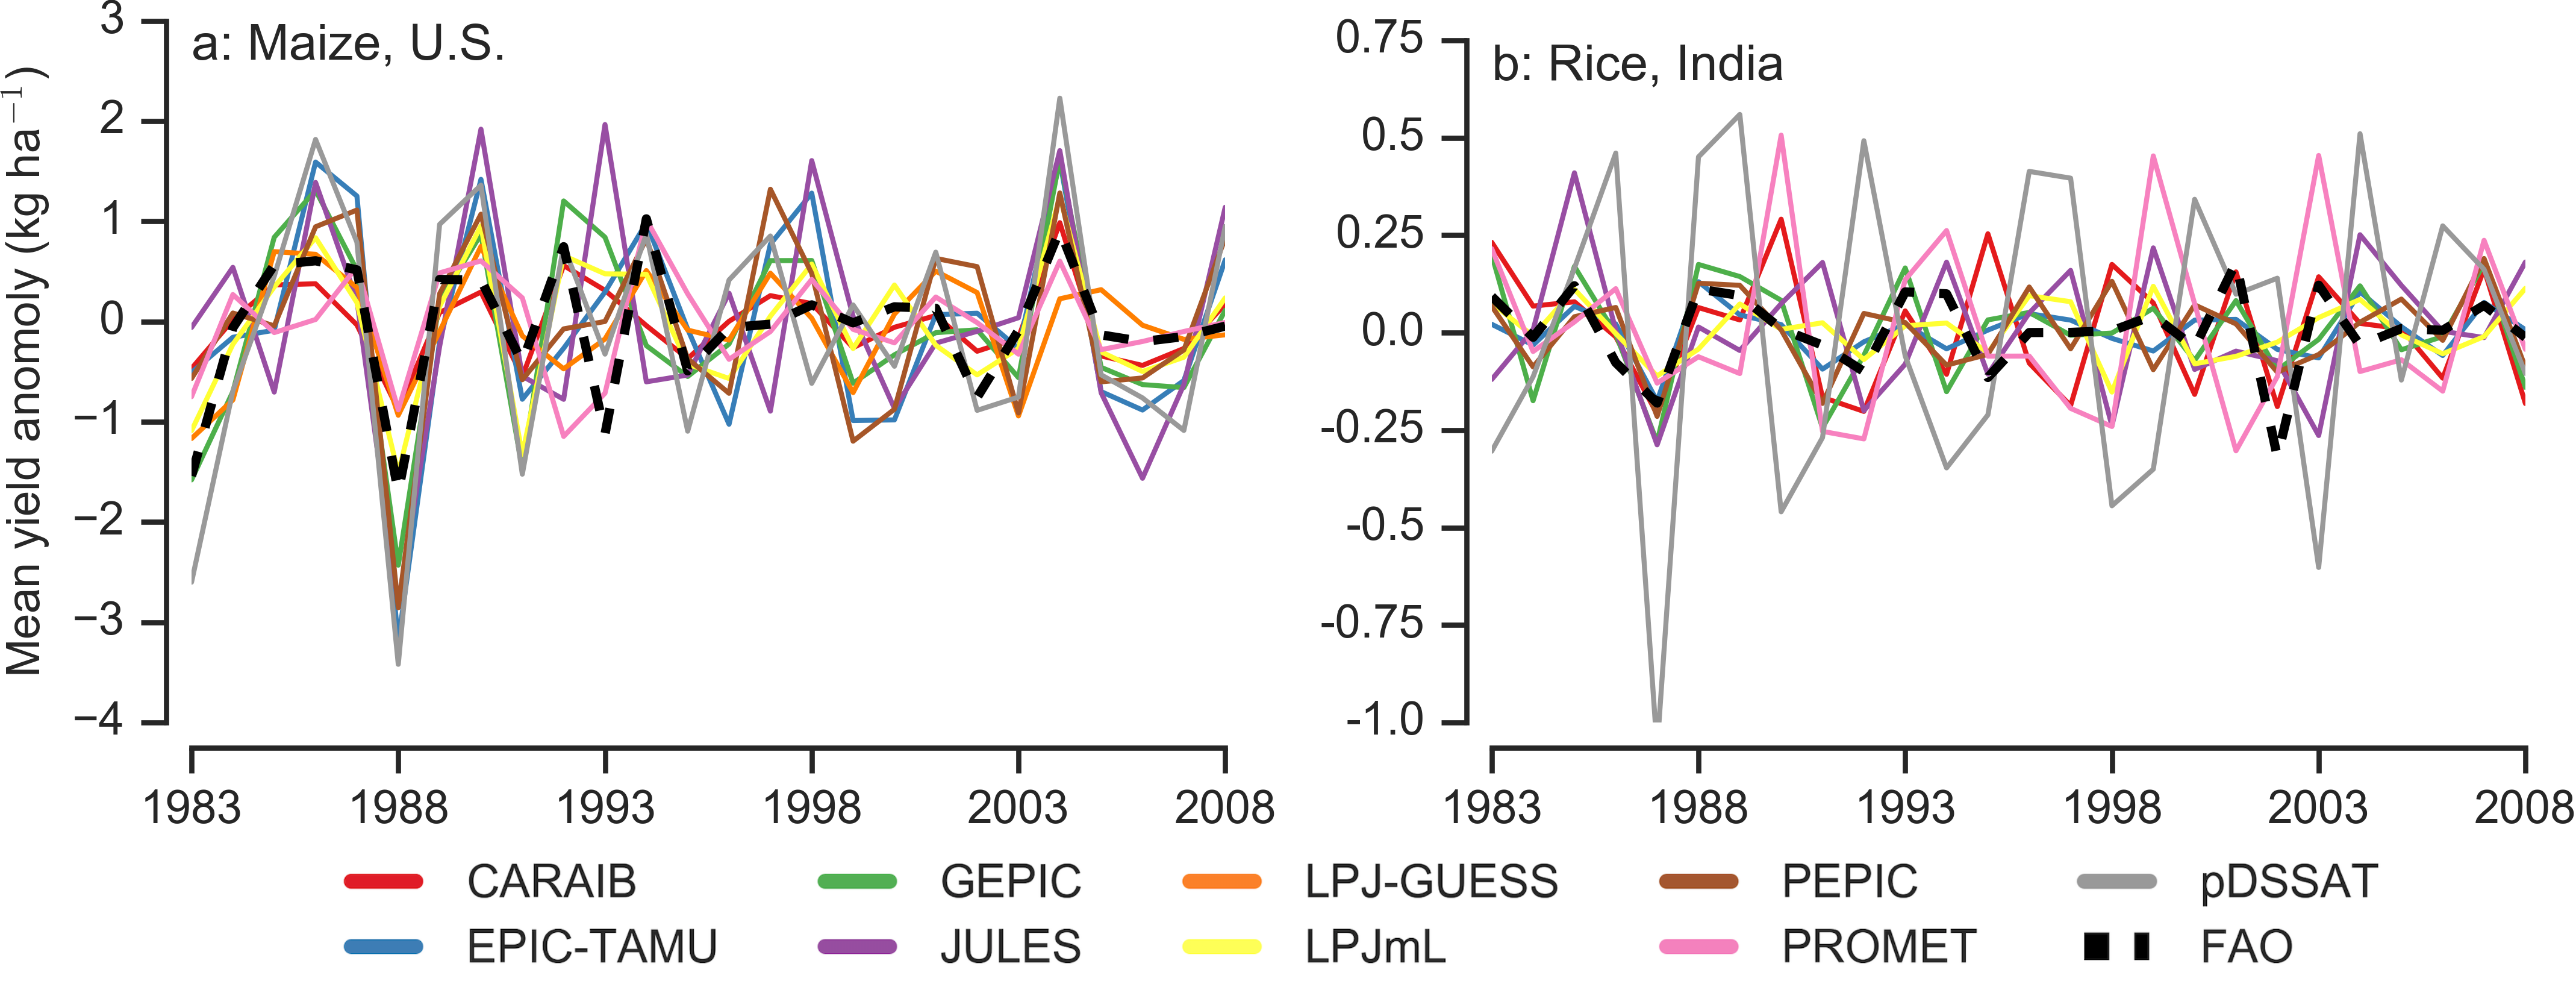
\includegraphics[width=14cm]{figures/validation_top.png}
  \includegraphics[width=14cm]{figures/validation_bottom1.jpg}
  \caption{
  Assessment of crop model performance in GGCMI Phase II, following the protocol of GGCMI Phase I \citep{muller_global_2017}. 
  \textbf{Top:} example timeseries comparison between simulated crop yield and FAO country statistics \citep{FAOSTAT} at the country level for two example high production countries: US maize, and rice in India, both for the 200 kg ha$^{-1}$ nitrogen application level. 
  \textbf{Bottom:} heatmaps illustrating the Pearson $r$ correlation coefficient between the detrended simulated and observed country-level mean yields for the top 10 countries by production for each crop, of those countries with continuous FAO data over 1981-2010.
  We show separate comparisons for simulations with the three different nitrogen application levels, denoted ``low'', ``med'', and ``high'' for 10, 60, and 200 kg N ha$^{-1}$, respectively. 
  Left column shows correlation of ensemble mean yields with FAO data 
  Because FAO does not distinguish between wheat types, we sum simulated spring and winter wheat for models that provide both (See Table \ref{table:models}.). 
  Note that differences by region and crop are stronger than difference between models, e.g.\ horizontal bars are more similar in color than vertical bars.
  }
  \label{fig:simulation_val}
\end{figure*}

%Generally, maize, wheat and soybean simulations of many GGCMs are capable of reproducing larger parts of observed temporal variability (time series correlation coefficients (r) of up to 0.888 for maize (Figure \ref{fig:ggcmi_phase1_eval}, reproduced from \cite{muller2016global}), 0.673 for wheat and 0.643 for soybean at the global scale)

Evaluating the performance of crop models in the GGCMI Phase II archive is complicated by the artificial nature of the protocol: the settings in the CTWN-A experiment design do not reflect actual conditions in the real world. 
The protocol includes one scenario of near-historical climate inputs (T$_0$, W$_0$, C$_{360}$), but the prescribed uniform nitrogen application levels do not reflect real-world fertilizer practices. Models also omit detailed calibrations to reflect the performance of historical cultivars. 

We provide a partial evaluation of the models’ skill in reproducing crop yield characteristics using the methodology of \citet{muller_global_2017}, developed for GGCMI Phase I.
\citet{muller_global_2017} evaluate how well model crop yield responses in a historical run capture real-world yield variations driven by year-to-year temperature and precipitation variations. 
Following this approach, we compare yields in the GGCMI Phase II baseline simulations with detrended historical yields from the Food and Agriculture Organization of the United Nations \citep{FAOSTAT} by calculating the Pearson product moment correlation coefficient. 
The procedure is sensitive to the detrending method and the area mask used to aggregate yields; we use a 5-year running mean removal and the MIRCA2000 cultivation area mask for aggregation. 
In some cases the model timeseries are shifted by one year to account for discrepancies in FAO or model year reporting. 
Because the GGCMI Phase II protocol imposes fixed, uniform nitrogen application levels that are not realistic for individual countries, we evaluate control runs for each model at multiple N levels whenever possible. 
Nine of the GGCMI Phase II models (Table 3) provide historical runs for all three nitrogen levels (10, 60, and. 200 kg ha$^-1$ yr$^-1$).

As expected due to the unrealistic features described above, correlation coefficients for the GGCMI Phase II simulations are slightly lower than those found in the Phase I evaluation, but models show reasonable fidelity at capturing year-over-year variation (Figure \ref{fig:simulation_val}). 
(Compare to \citet{muller_global_2017} Figures 1--4 and 6.)  
Differences in fidelity between regions and crops exceed differences between models: 
that is, Figure \ref{fig:simulation_val} shows more color similarity in horizontal than vertical bars. 
For example, maize in the United States is consistently well-simulated while maize in Indonesia is problematic (mean Pearson correlation coefficients of 0.68 and 0.18, respectively). 
Note that in this methodology, simulations of crops with low year-to-year variability such as irrigated rice and wheat will tend to score more poorly than those with higher variability.
In some cases, especially in the developing world, low correlation coefficients may point to reporting problems in the FAO statistics \citep{Ray2012, muller_global_2017}. 
No single model consistently exhibits greater fidelity than others. 
Instead, each model shows near best-in-class performance for at least one location-crop combination. 
For example, pDSSAT is the best model for maize in the US, LPJmL and GEPIC are best in Germany, PROMET is best in Argentina, and PEPIC and LPJ-GUESS are best in France.

\subsection{Model crop yield responses under CTWN forcing}
\begin{figure*}[ht]
\centering
  \includegraphics[width=14cm]{figures/baselinecomp_yield_5.png} 
  \caption{
  Illustration of the spatial patterns of potential yields (left) and yield changes (right) in the GGCMI Phase II ensemble. 
  Left column shows multi-model mean climatological potential yields for the baseline scenario, with white stippling indicating areas where these crops are not currently cultivated. 
  Absence of cultivation aligns well with the lowest yield contour (0-2 ton ha$^{-1}$). 
  Right column shows multi-model mean fractional yield changes in the T+4 $^{\circ}$C scenario relative to the baseline scenario. 
  Areas without stippling are those where models agree on changes: the multi-model mean fractional change exceeds the standard deviation of changes in individual models. 
  Stippling indicates areas of low confidence ($\Delta < 1 \sigma$). 
  Some spatial structure in projected changes at high latitudes may be due to differences in model coverage; see Figure \ref{fig:crop_area}.
  }
  \label{fig:maizesoybaseline}
\end{figure*}

\begin{figure*}[ht]
\centering
  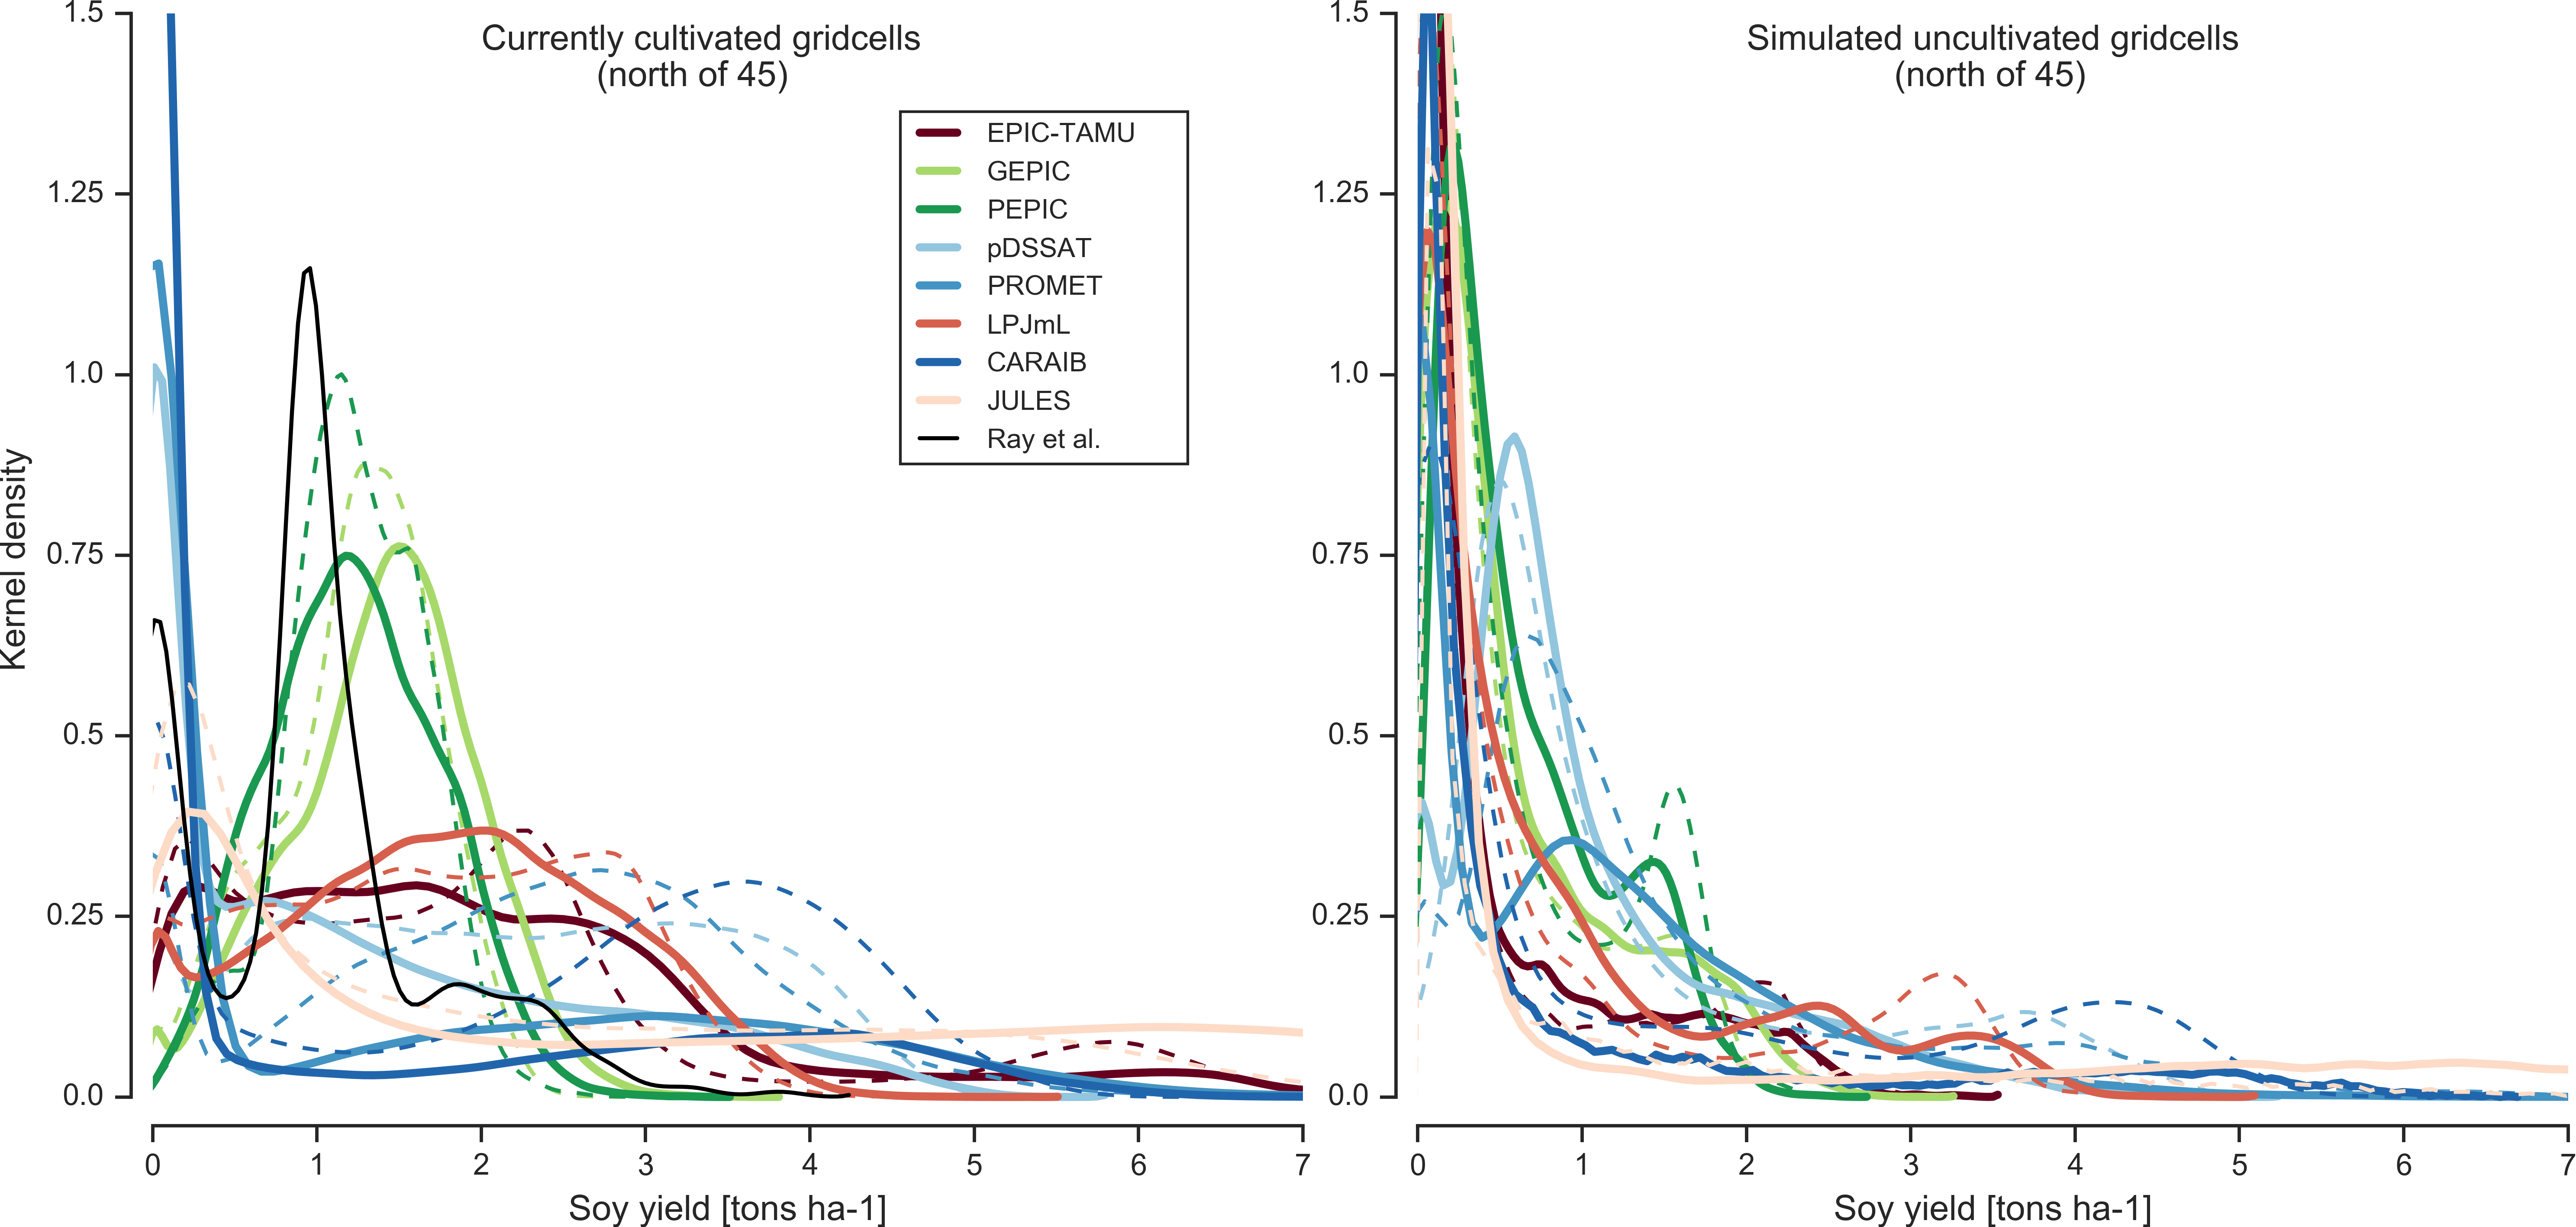
\includegraphics[width=15cm]{figures/soy_highlats.png}
  \caption{
  Model probability densities for soybean yields at latitudes north of 45$^\circ$ in historical and warming simulations in the A0 case. 
  While all 11 GGCMIP Phase II models provide simulations; we show 8 representative models for clarity.
  Probability density functions are estimated separately for locations with some current cultivation (left, approximately 2500 grid cells, unweighted by cultivated area) and for uncultivated locations (right, approximately 1500 grid cells), for baseline historical (solid) and T+4 (K) (dashed) simulations. 
  Black line in left panel shows actual yields from 1997-2003 derived from \cite{Ray2012}. 
  For historical simulations, models agree on low potential yields in currently uncultivated areas (right) but disagree widely on yields in currently cultivated areas (left). 
  Color code groups models into those with realistic yield distributions peaking at 1-2 ton ha$^{-1}$ (green), those with flatter distributions extending to unrealistically high values (red), and those with predominantly zero yields (blue). 
  ``Green'' models show slight decreases under T+4 warming, ``red'' models moderate increases, and ``blue'' models large increases. 
  }
\label{fig:highlat}
\end{figure*}

\begin{figure*}[ht]
  \centering
  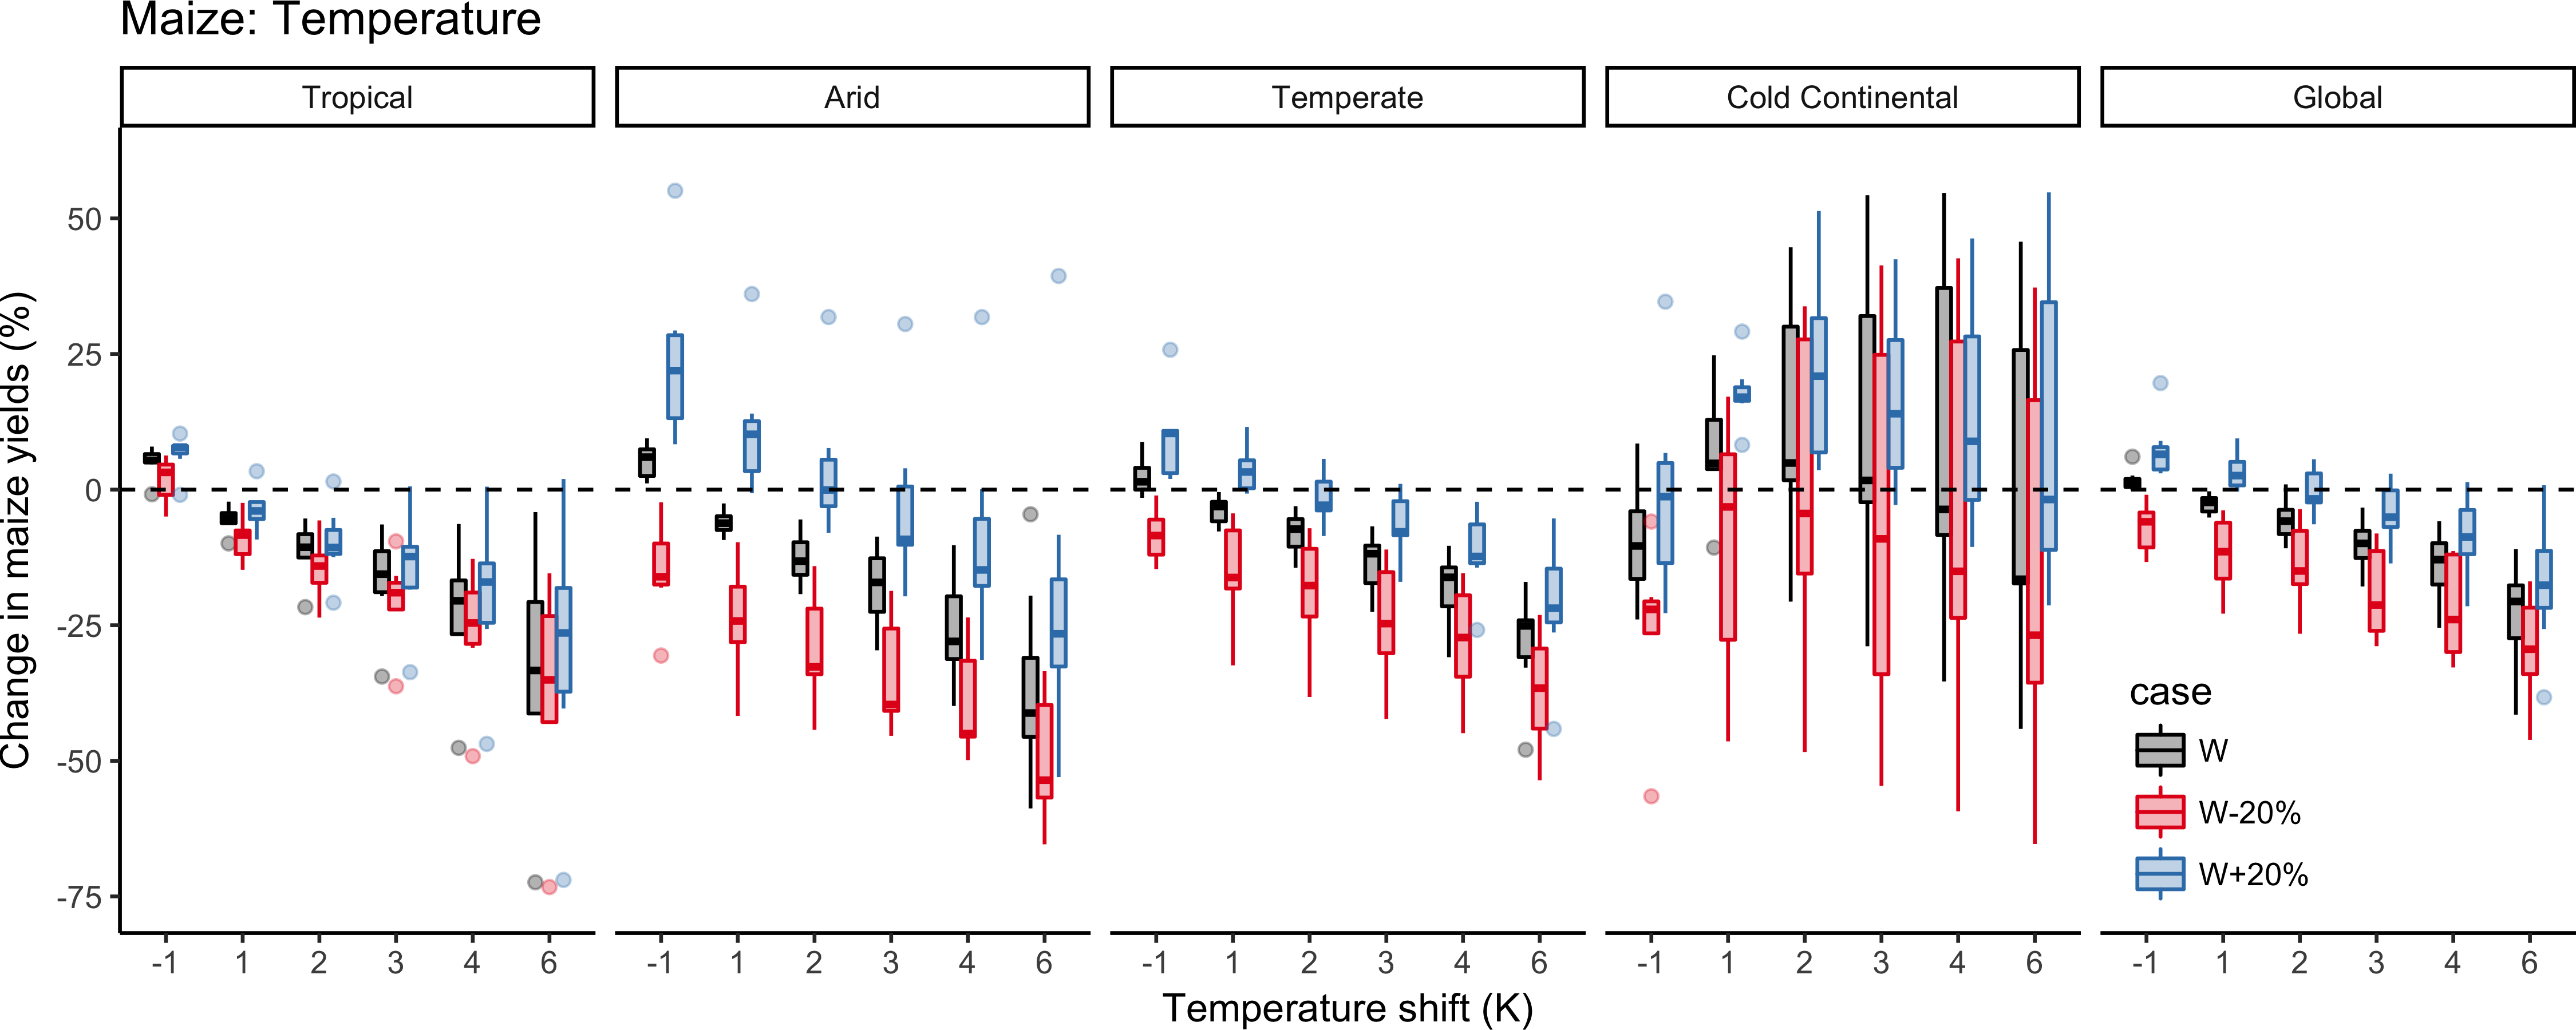
\includegraphics[width=15cm]{figures/maize_sim_CG_T.png}
  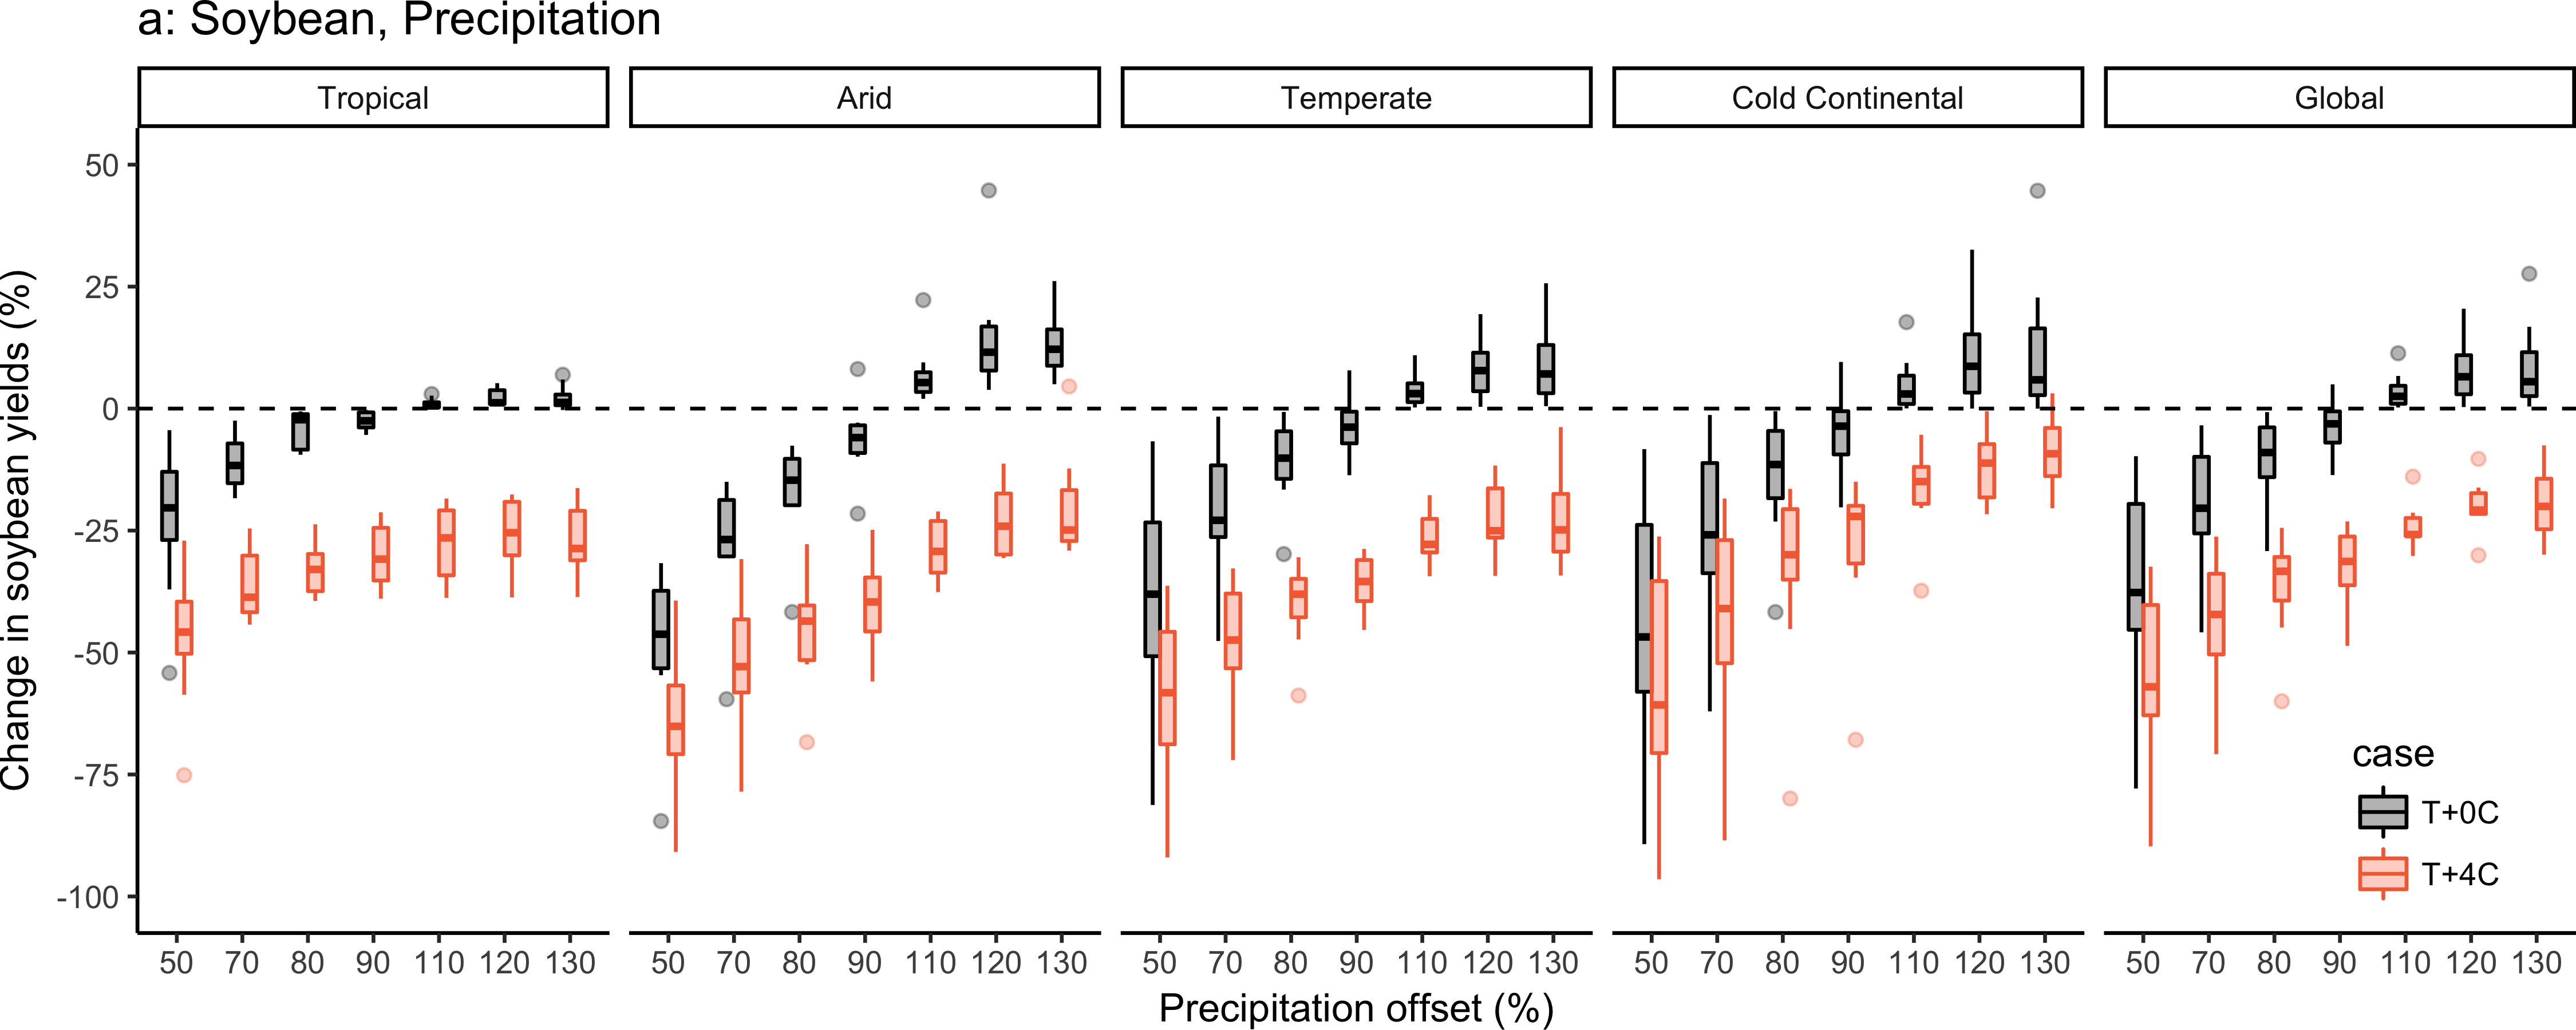
\includegraphics[width=15cm]{figures/soy_sim_CG_W.png}
  \caption{
  Illustration of the distribution of regional yield changes across the multi-model ensemble, split by K\"{o}ppen-Geiger climate regions, and with global response in rightmost panel.
  Y-axis is the fractional change in the regional average climatological (30-year mean) potential yield relative to the baseline.
  Box-and-whiskers plots show distribution across models, with median marked; edges are first and third quartiles and whiskers extend to 1.5$\cdot$IQR.
  Figure shows all all simulated grid cells for each model; see Supplemental Figure S10-S13 for only currently-cultivated land. We highlight responses to individual factors; note that results are not directly comparable to simulations of realistic climate scenarios with identical global mean changes.  
  Models generally agree outside high-latitude regions, with projected changes exceeding inter-model variance.
  \textbf{Top:} Response of rainfed maize to applied uniform temperature perturbations, for three discrete precipitation perturbation levels ( -20\%, 0\%, and +20\%), with CO$_2$ and nitrogen held constant at baseline values (360 pmm and 200 kg ha$^{-1}$ yr$^{-1}$).
  Outliers in the tropics (strong negative impact of higher T) are the pDSSAT model; outliers in the arid region (strong positive impact of higher P) are JULES.
  \textbf{Bottom:} 
  Response of rainfed soybeans to applied uniform precipitation perturbations, for two discrete temperature levels.
  Cases with reduced precipitation show greater inter-model spread than those with increased precipitation.
  At very large precipitation increases, yield changes level out: benefits saturate once water availability is no longer limiting.
  Precipitation changes are more important in the arid region, as expected. 
  Note the large uncertainty in the cold continental region, also illustrated in Figures 3 and 4.
  }
  \label{fig:maizerice}
\end{figure*}


\begin{figure*}[ht]
  \centering
  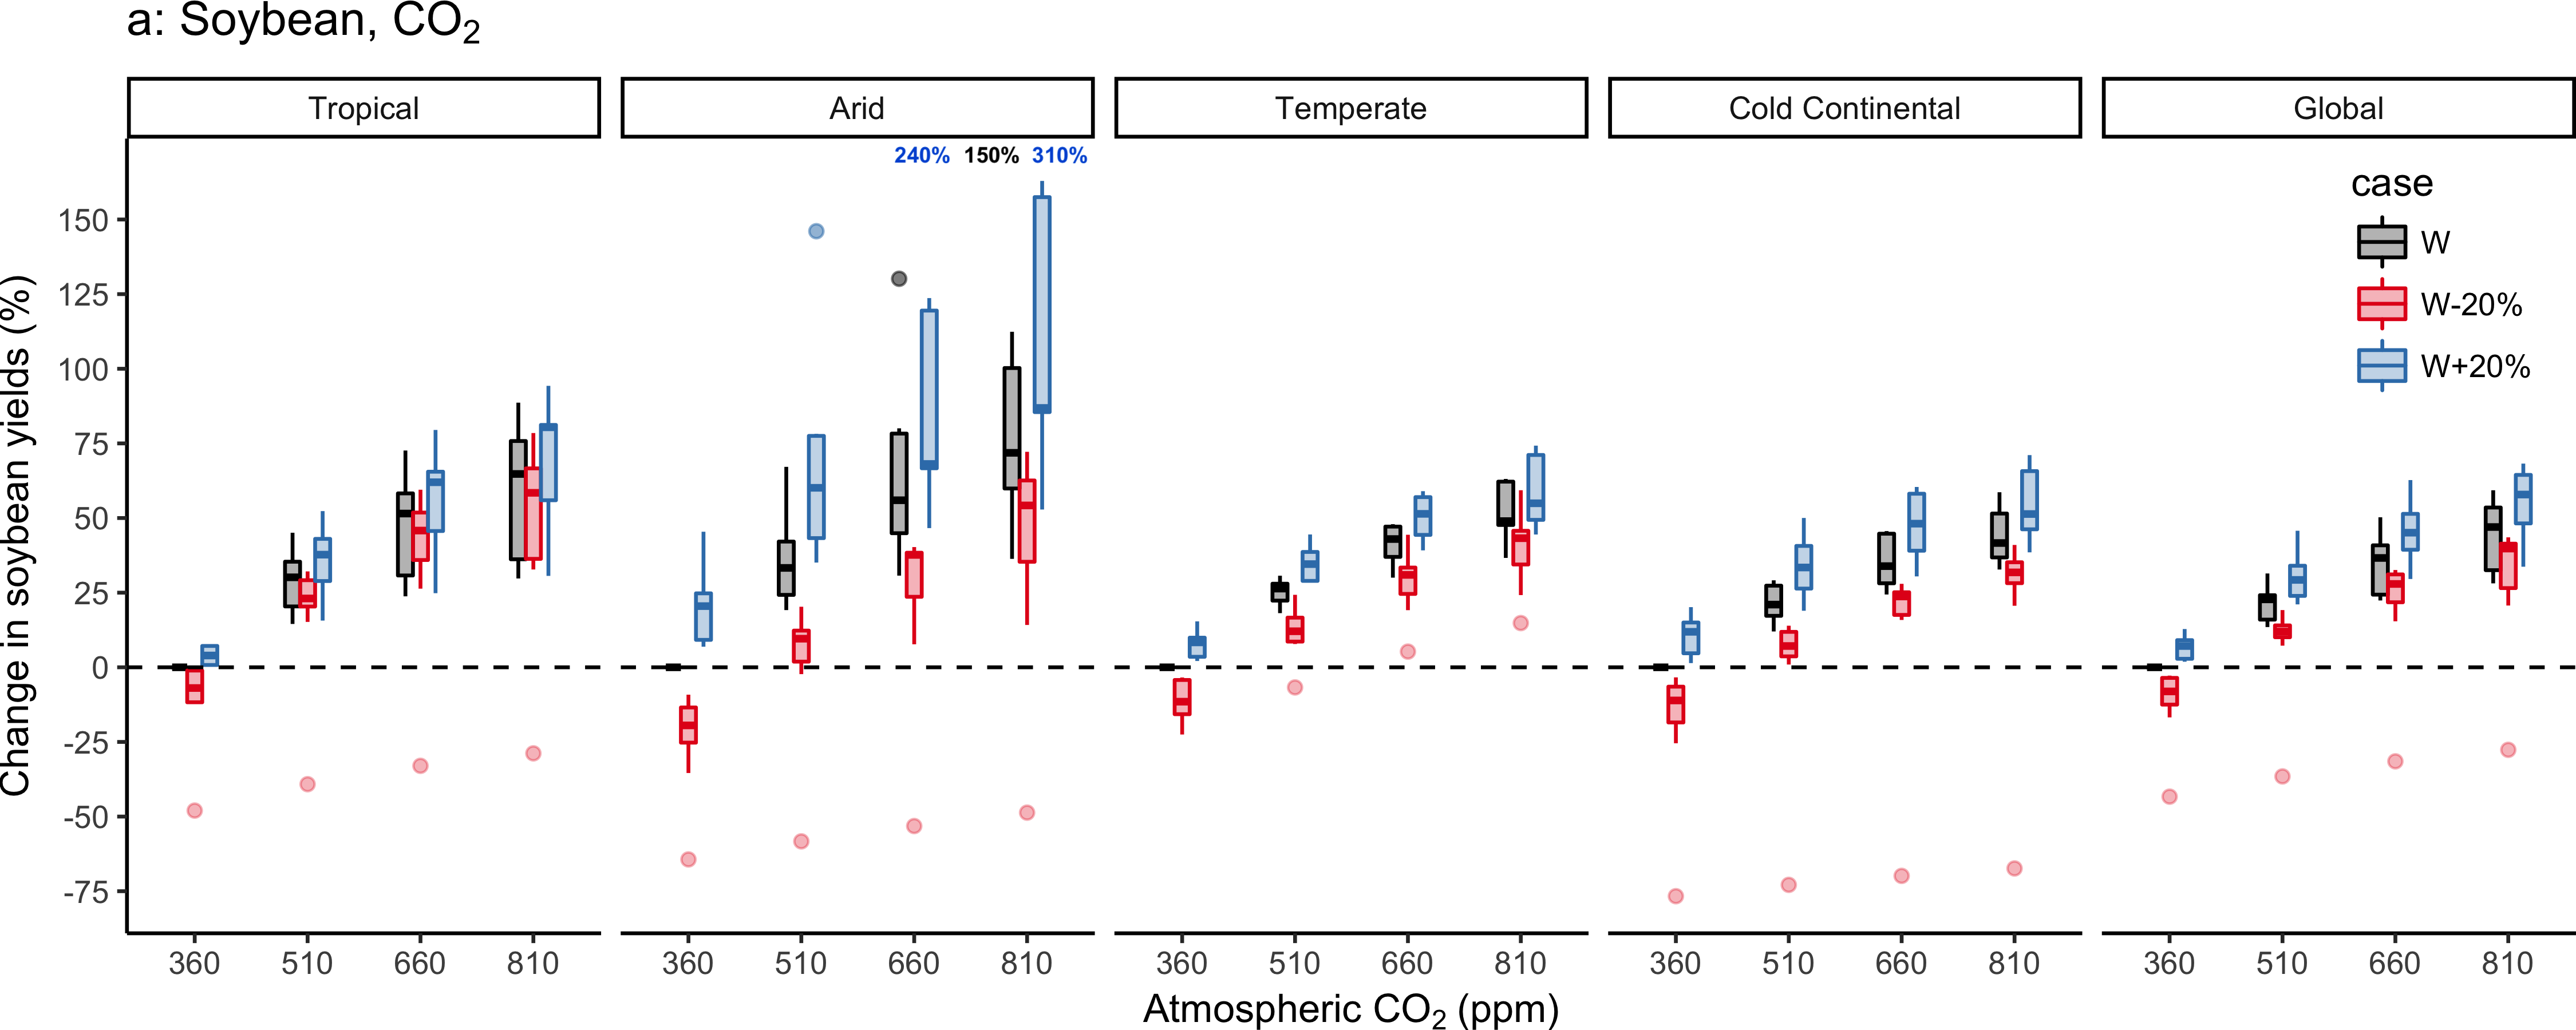
\includegraphics[width=15cm]{figures/soy_sim_CG_C.png}
  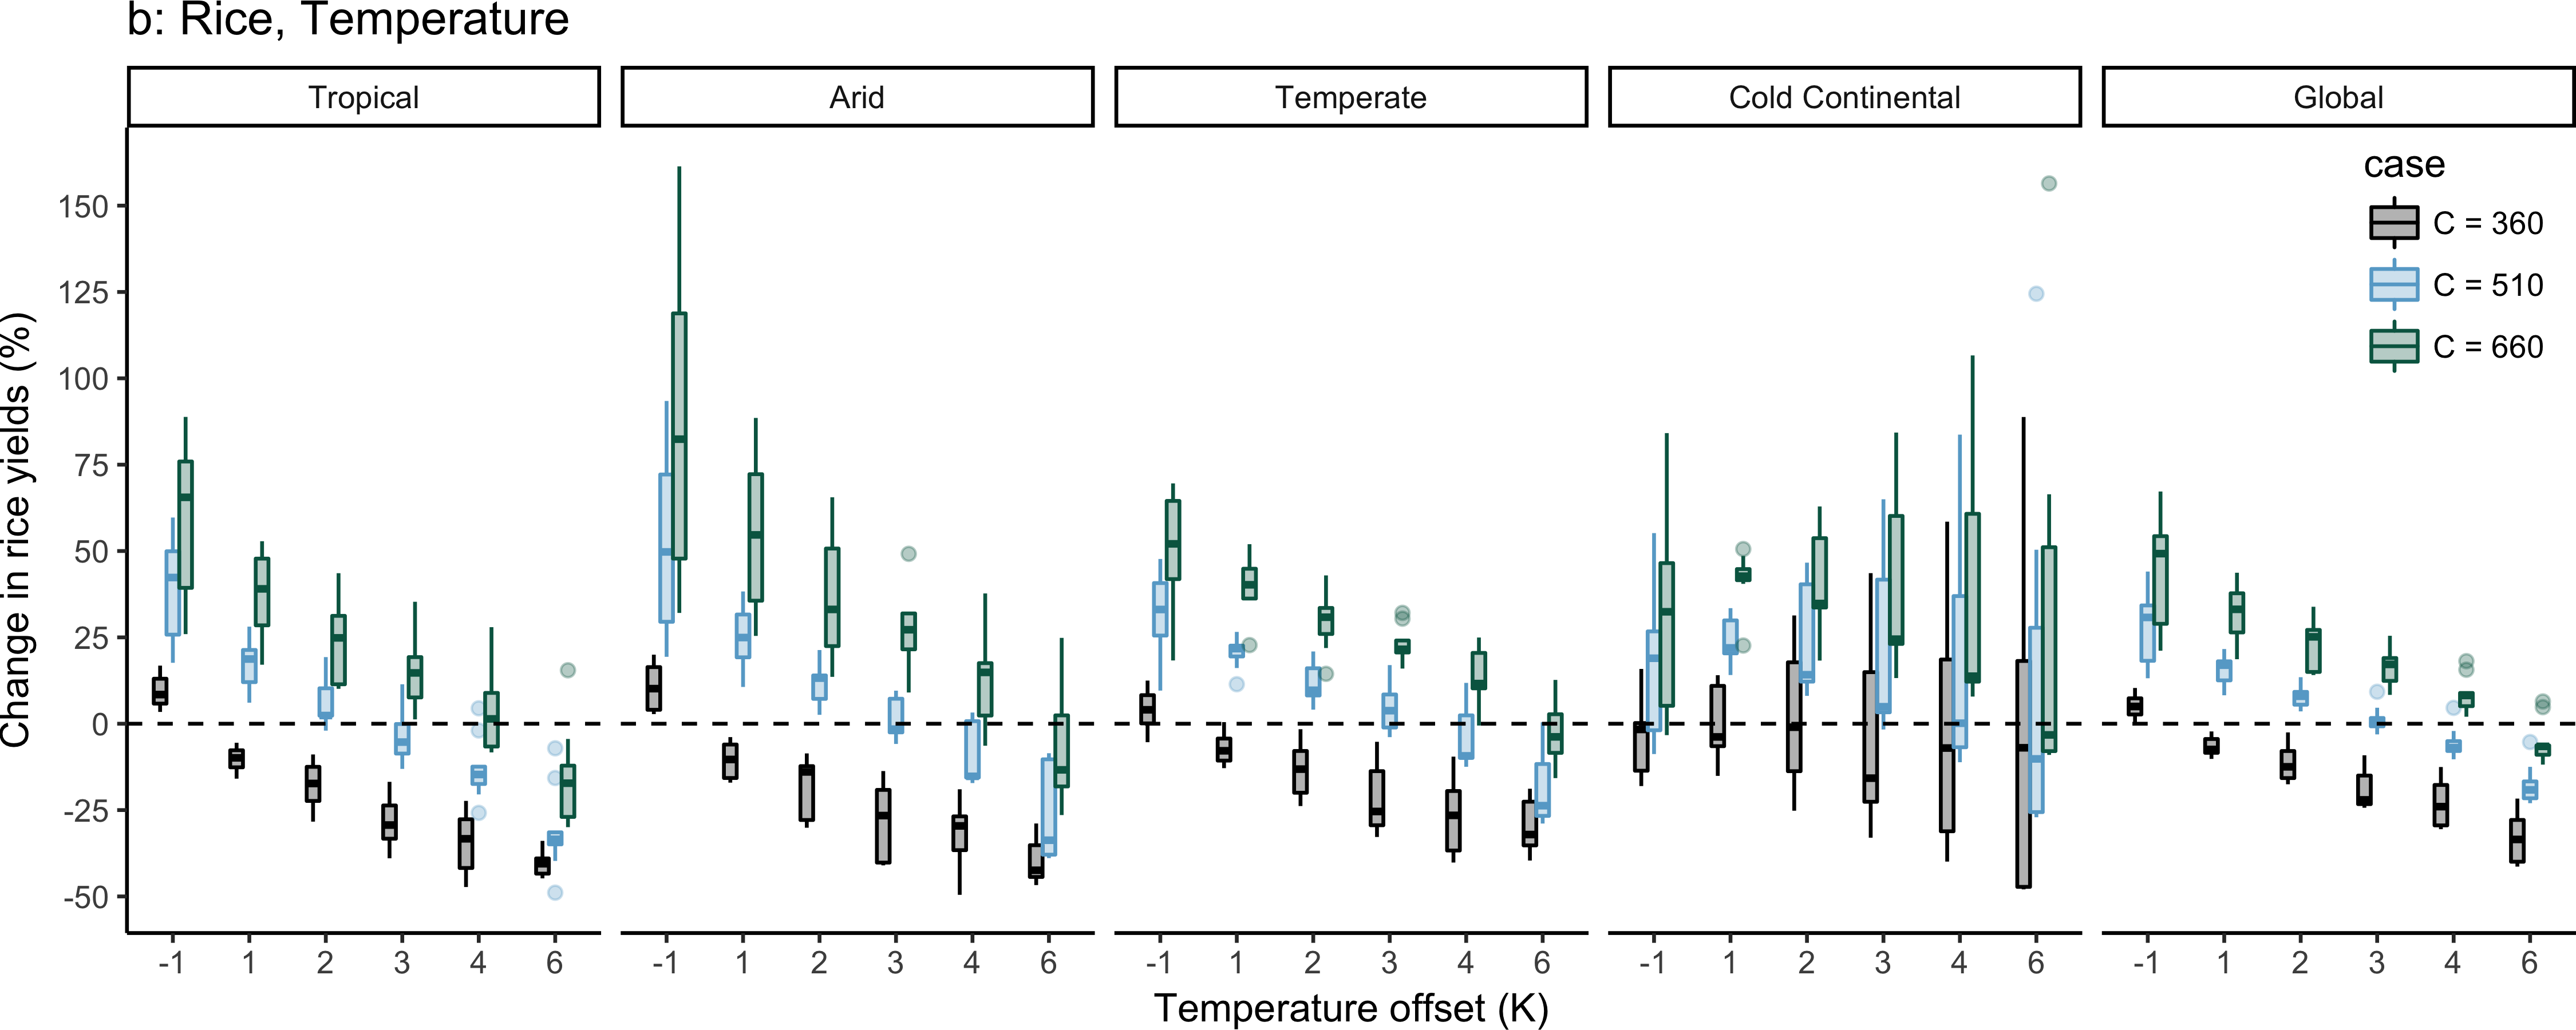
\includegraphics[width=15cm]{figures/rice_sim_CG_T.png}
  \caption{
  Illustration of the distribution of regional yield changes across the multi-model ensemble, here for soybeans and rice for the A0 case. Conventions as in Figure \ref{fig:maizerice}.
  \textbf{Top:} 
  Response of rainfed soybeans to atmospheric CO$_2$, for three discrete precipitation perturbation levels with temperature and nitrogen held constant at baseline values.
  Low outliers are the EPIC-TAMU model and the high outliers in the Arid region are the JULES model.
  Reduced precipitation tends to steepen the CO$_2$ response and increased precipitation tends to flatten it, as expected. 
  Reduced precipitation tends to increase the inter model spread, especially at the highest CO$_2$ levels.
  \textbf{Bottom:} 
  Response of irrigated rice for three discrete CO$_2$ levels, with nitrogen and precipitation held constant. 
  CO$_2$ does not change the nature of temperature response respective to baseline as the slopes at each CO$_2$ level are relatively constant.
  }
  \label{fig:soywheat}
\end{figure*}

Crop models in the GGCMI Phase II ensemble show broadly consistent responses to climate and management perturbations in most regions, with a strong negative impact of increased temperature in all but the coldest regions. 
Mapping the distribution of baseline yields and yield changes shows the geographic dependencies that underlie these results. 
Absolute yield potentials show strong spatial variation, with much of the Earth's surface area unsuitable for any of these crops (Figure \ref{fig:maizesoybaseline}, left).
Crop yield changes under climate perturbations also show distinct geographic patterns (Figure \ref{fig:maizesoybaseline}, right, which shows fractional yield differences between the T+4 scenario and the baseline scenario with historical climatology).
In general, models agree most on yield response in regions where yield potentials are currently high and therefore where crops are currently grown. 
Models show robust decreases in yields at low latitudes, and highly uncertain ensemble mean increases at most high latitudes.

Projections of strong yield growth at higher latitudes should be treated with caution, since the effects evident in Figure \ref{fig:maizesoybaseline} are due in part to inaccuracies in model representations of present-day crop yields. 
For example, at latitudes north of 45$^\circ$, the GGCMI Phase II models collectively suggest strong (but uncertain) growth in soybean yields under warmer conditions (Figure \ref{fig:maizesoybaseline}, g). 
However, model differences are greater in the baseline than future simulations, and greatest in currently-cultivated areas (Figure \ref{fig:highlat}). 
Both the mean projected growth and the inter-model spread are driven by three models that show almost zero present-day potential soybean yields across the entire high-latitude region, even in locations where soybeans are currently grown (Figure \ref{fig:highlat}, left).
PROMET, for example, involves a stronger response to cold than other models (e.g.\ LPJmL) with frost below -8 $^\circ$C irreversibly killing non-winter crops and prolonged periods of below-optimum temperatures also leading to complete crop failure. 
Over the high-latitude regions simulated by both models, 52\% of grid cells in PROMET report 0 yield in the present climate vs. 
11\% of cells in the T+4 scenario, leading to a strong yield gain in warmer future climates. 
In LPJmL outputs, the same high-latitude area is deemed suitable for cultivation even in baseline climate, with crop failure rates of 4\% and 5\% in present and T+4 cases, so that projected yield changes are modest (Figure \ref{fig:highlat}).
These spurious low baseline yields result in very large fractional changes in the T+4 warming scenario, when all models agree that conditions become favorable for soybeans. 
Those models that most accurately reproduce present-day high-latitude soybean yields of 1-2 ton ha$^{-1}$ \citep{Ray2012} in fact show a slight decrease in yield under a warming scenario (Figure \ref{fig:highlat}, left). 
Apparent future yield increases in the multi-model mean are driven by the least realistic simulations.

The GGCMI Phase II exercise offers the opportunity to examine and characterize not just crop response to a single temperature change but nonlinearities in responses and interactions between factors. 
We illustrate a few of these relationships in Figures 5—6, choosing crops and factors whose effects are reasonably well understood. 
It is expected, for instance, that increases in precipitation should buffer the effects of warmer temperatures and that CO$_2$f increases should reduce damage to crops in scenarios where water is limited. 
Models generally confirm expected behavior but also provide insight into unforeseen interactions. 
To show geographic effects, we divide model responses in Figures \ref{fig:maizerice}—\ref{fig:soywheat} by the primary K\"{o}ppen-Geiger climate regions \citep{rubel2010}, showing the yield changes across all simulated grid cells in each region. 
In each panel we examine relationships between two factors, showing yield response against one for several scenarios of the other, in box plots that show the inter-model spread. 
The responses highlighted here are qualitatively similar across all crops included in this study (Supplemental Figures S5 - S8). 

For all crops, warming scenarios with precipitation held constant produce yield decreases in most regions. 
These impacts are robust for even moderate climate perturbations. For rainfed maize, even a 1 degree temperature increase with other factors held constant produces a median regional decline in potential yield that exceeds the variance across models, in all but the ``cold-continental'' regions (Figure \ref{fig:maizerice}a). 
The remaining areas (‘warm temperate’, ‘equatorial’, and ‘arid’) account for nearly three-quarters of global maize production. In the high-latitude ``cold-continental'' region, potential yield changes are positive but highly uncertain, for the reasons discussed previously; uncertainties are larger even for maize than for soybeans. 
(Compare Figures \ref{fig:maizerice}a and \ref{fig:maizerice}b.) 
Temperature effects are somewhat nonlinear, with the largest impacts for maize in the warm ``tropical'' region. 
(For soybeans, temperature effects are more complex; see Supplemental Figure S5.) 
Precipitation effects on rainfed crops are more strongly nonlinear. 
The curvature of the precipitation response can be seen by eye in Figure \ref{fig:maizerice}b: soybean yields are strongly negatively impacted by reduced rainfall, peak under increased precipitation of 20\%, and actually decline at higher precipitation levels. 

As expected, precipitation and temperature effects interact, with increases in precipitation buffering yield responses to temperature. 
Increased rainfall mitigates the negative impacts of warmer temperatures caused by increased evapo-transpiration (cite). 
For maize, the effect is relatively modest outside the ``arid'' regions (Figure \ref{fig:maizerice}a). 
Globally, a 4 degree temperature rise with no change in precipitation results in median loss of $\sim$13\% of rainfed maize, with all models showing a negative response.
With a 20\% increase in precipitation, the median yield loss is $\sim$8\%. 
For soybeans, the equivalent values are $\sim$11\% and 1\%, respectively. 
Decreased rainfall, on the other hand, amplifies yield losses and also increases inter-model variance. 
That is, models agree that the response to decreased water availability is negative in sign but disagree on its magnitude. 
Outside of arid regions, the interaction effect itself shows little nonlinearity (i.e. response slopes in Figures \ref{fig:maizerice}a and \ref{fig:maizerice}b are roughly parallel). 
As expected, irrigated crops are more resilient to temperature increases in all regions, especially so where water is already limiting (other than winter wheat, Supplemental Figure S9).

Increased CO$_2$ boosts yields overall through the well-known CO$_2$ fertilization effect (Figure \ref{fig:soywheat}). 
The effect is strongest for the C3 crops (wheat, soybeans, and rice), while maize, a C4 grass, has a comparatively muted response. 
We show irrigated rice and rainfed soy in Figure \ref{fig:soywheat} as representative C3 crops.  
The effect of CO$_2$f on yields is nonlinear, as expected, with significant benefit from small increases but with effects plateauing at higher concentrations (Figure \ref{fig:soywheat}). 
CO$_2$ and temperature effects show minimal interaction. 
This effect is seen in Figure \ref{fig:soywheat}a, which shows nearly parallel response slopes at different CO$_2$ levels. 
That is, CO$_2$ fertilization does little to change the nature of the temperature response. 
On the other hand, CO$_2$ and precipitation effects interact strongly, as expected since higher CO$_2$ levels allow reduced stomatal conductance and evapotranspiration losses, mitigating the effect of reduced rainfall. 
This interaction is seen in Figure \ref{fig:soywheat}b as smaller yield losses from reduced rainfall when CO$_2$ levels are higher. 
For example, for soy, raising CO$_2$ to 510 ppm actually outweighs the multi-model median damages caused by a 20\% precipitation reduction in all climate regions. 
All crops show similar behavior, but note that model uncertainties for wheat are substantially higher than those for other crops, possibly because model calibration is especially important for wheat \citep{Asseng2013}. 
(Compare Figure \ref{fig:soywheat}a for soy and Supplemental Figure S7 for wheat).

\section{Discussion and Conclusions} 
\label{S:5}
The GGCMI Phase II experiment provides a database designed to allow detailed study of multi-factor crop yields in process-based models under climate change. While previous crop model intercomparison projects in the climate change context have focused on simulations along realistic climate scenarios,
the use of systematic input parameter variations in GGCMI Phase II (with up to 756 scenarios) allows not only comparing yield sensitivities to changing climate and management inputs but also evaluating the complex interactions between important driving factors: CO$_2$, temperature, precipitation, and applied nitrogen. 
The global extent of the experiment also allows identifying geographic shifts in high potential yield locations. 
With 12 participating models and 31 simulation years per scenario the complete database constitutes over 150,000 years of global yield simulation output. 

Preliminary results shown here highlight some of the insights provided by the simulation exercise and lend confidence in the models.
First, in historical simulations, year-over-year correlations in modeled and actual country-level yields are generally good in most cases with with no single model dominating performance globally.
Second, models generally agree on changes driven by all factors outside the high latitudes (where models differ in treatment of crop response to current cold conditions).
Third, interactions between major yield drivers (temperature and precipitation in Figure \ref{fig:maizerice}, precipitation and CO$_2$ in Figure \ref{fig:soywheat}) generally follow expectations.

Users should be aware of some limitations with the experiment. 
First, absolute model yield values in the historical scenario will generally not match observed yields.  
In order to match current yields, process-based models must generally be re-tuned to account for the constant evolution of crop cultivar genetics and  management practice \citep[e.g.][]{JONES2017b}. The historical scenario also includes no trend in CO$_2$, and scenarios assume unrealistic globally uniform nitrogen application levels \citep{Elliott2015}.
%As our goal is testing model sensitivity to important
%% justification of why this choice was made and doesn't matter the purposes here - just want the changes, absolute level doesn't matter XX
However, note that the models used in this exercise cannot not simulate some climate-induced yield changes due to factors such as pests, diseases, and weeds. 
Second, exercise is intended to allow studying factors that will affect future yields, but no individual scenario in the exercise is itself a realistic future projection.
Uniform offsets in temperature and precipitation are not realistic because climate change will result in spatially heterogeneous changes mean temperature and precipitation. 
Using GGCMI Phase II simulation results for impacts projection requires the construction of an emulator of crop yield response to climatological changes. 
However, note that the experiment does not sample over potential changes in the higher-order moments in the distributions in temperature and precipitation. 

We expect that the simulations will yield multiple insights in future studies. 
Potential applications include emulators, yield response surface, adaptation studies, nitrogen use efficiency, regional production shifts, and others.
In general, the development of multi-model ensembles involving systematic parameters sweeps has large promise for increasing understanding of potential future crop responses and for improving process-based crop models.
We expect that the GGCMI Phase II data archive will be used to analyze the different GGCMs' sensitivity to changes in the CTWN-A space, including the interaction between drivers.

%%%%%%%%%%%%%%%%%%%%%%%%%%%%%%%%%%%%%%%%%%%%%%%%%%%%%%%%%%%%%%%
\begin{sloppypar}
\codedataavailability{The simulation outputs of the mandatory 7 output variables (Table \ref{table:outputs}) are available on zenodo.org. 
See Appendix \ref{A:1} for data DOIs. 
All other simulation output variables are available upon request to the corresponding author. 
The scripts for generating the spring wheat and winter wheat growing seasons and second fertilizer dates and the quality screening script is available at https://github.com/RDCEP/ggcmi/blob/phase2/.
All input data are available via globus.org (registration required, free of charge):
Minimum cropland mask is available at
\url{https://app.globus.org/file-manager?origin_id=e4c16e81-6d04-11e5-ba46-22000b92c6ec&origin_path=\%2FAgMIP.input\%2Fother.inputs\%2Fphase2.masks\%2F}
choose the file boolean\_cropmask\_ggcmi\_phase2.nc4
Growing period data for wheat is now divided up into winter and spring wheat, available at
\url{https://app.globus.org/file-manager?origin_id=e4c16e81-6d04-11e5-ba46-22000b92c6ec&origin_path=\%2FAgMIP.input\%2Fother.inputs\%2FAGMIP_GROWING_SEASON.HARM.version2.0\%2F}
whereas all other growing season data (maize, rice, soybean) are the same as in Phase I (version 1.25), available at
\url{https://app.globus.org/file-manager?origin_id=e4c16e81-6d04-11e5-ba46-22000b92c6ec&origin_path=\%2FAgMIP.input\%2Fother.inputs\%2FAGMIP_GROWING_SEASON.HARM.version1.25\%2F}
}
\end{sloppypar}

\appendix
\section{}
\subsection{Data Access}
\label{A:1}
Simulation yield output datasets can be found at the DOIs located in table \ref{table:dataloc}. 
Data are published in crop- and GGCM-specific packages, in order to break down the overall data amount into manageable packages (<50GB per archive).

\begin{table*}[t]
  \caption{DOI's for model data outputs. All model output data can be found at https://doi.org/10.5281/zenodo/XX. Where XX is the value listed in the table.} 
  \label{table:dataloc}
  \begin{tabular}{p{3cm} p{1.5cm} p{1.5cm} p{1.5cm} p{1.5cm} p{1.5cm}}
    \tophline
    {\textbf{Model}}&{\textbf{Maize}}&{\textbf{Soybean}}&{\textbf{Rice}}&{\textbf{Winter wheat}}&{\textbf{Spring wheat}}\\ \middlehline
    {\textbf{APSIM-UGOE}} & {2582531} & {2582535} & {2582533} & {2582537} & {2582539}\\ \middlehline
    {\textbf{CARAIB}} & {2582522} & {2582508} & {2582504} & {2582516} & {2582499}\\ \middlehline
    {\textbf{EPIC-IIASA}} & {2582453} & {2582461} & {2582457} & {2582463} & {2582465}\\  \middlehline
    {\textbf{EPIC-TAMU}} & {2582349} & {2582367} & {2582352} & {2582392} & {2582418}\\ \middlehline
    {\textbf{JULES}} & {2582543} & {2582547} & {2582545} & {--} & {2582551}\\ \middlehline
    {\textbf{GEPIC}} & {2582247} & {2582258} & {2582251} & {2582260} & {2582263}\\ \middlehline
    {\textbf{LPJ-GUESS}} & {2581625} & {--} & {--} & {2581638} & {2581640}\\  \middlehline
    {\textbf{LPJmL}} & {2581356} & {2581498} & {2581436} & {2581565} & {2581606}\\ \middlehline
    {\textbf{ORCHIDEE-crop}} & {2582441} & {--} & {2582445} & {2582449} & {--}\\ \middlehline
    {\textbf{pDSSAT}} & {2582111} & {2582147} & {2582127} & {2582163} & {2582178}\\ \middlehline
    {\textbf{PEPIC}} & {2582341} & {2582433} & {2582343} & {2582439} & {2582455}\\ \middlehline
    {\textbf{PROMET}} & {2582467} & {2582488} & {2582479} & {2582490} & {2582492}\\
    \bottomhline
  \end{tabular}
\end{table*}
\noappendix %% use this to mark the end of the appendix section

\authorcontribution{J.E., C.M, and A.R.\ designed the research. C.M., J.J., J.B., P.C., M.D., P.F., C.F., L.F., M.H., C.I., I.J., C.J., N.K., M.K., W.L., S.O., M.P., T.P., A.R., X.W., K.W., and F.Z.\ performed the simulations. J.F., J.J., C.M., and E.M.\ performed the analysis and J.F., E.M., and C.M.\ prepared the manuscript.}

\competinginterests{The authors declare no competing interests.}

\begin{acknowledgements}
This research was performed as part of the Center for Robust Decision-Making on Climate and Energy Policy (RDCEP) at the University of Chicago, and was supported through a variety of sources. 
RDCEP is funded by NSF grant \#SES-1463644 through the Decision Making Under Uncertainty program. 
J.F.\ was supported by the NSF NRT program, grant \#DGE-1735359. 
C.M.\ was supported by the MACMIT project (01LN1317A) funded through the German Federal Ministry of Education and Research (BMBF). 
C.F.\ was supported by the European Research Council Synergy grant \#ERC-2013-SynG-610028 Imbalance-P. 
P.F.\ and K.W.\ were supported  by the Newton Fund through the Met Office Climate Science for Service Partnership Brazil (CSSP Brazil). 
K.W.\ was supported by the IMPREX research project supported by the European Commission under the Horizon 2020 Framework programme, grant \#641811. 
A.S.\ was supported by the Office of Science of the U.S. Department of Energy as part of the Multi-sector Dynamics Research Program Area. 
S.O.\ acknowledges support from the Swedish strong research areas BECC and MERGE together with support from LUCCI (Lund University Centre for studies of Carbon Cycle and Climate Interactions). 
R.C.I.\ acknowledges support from the Texas Agrilife Research and 634 Extension, Texas A \& M University. This is paper number 35 of the Birmingham Institute of Forest Research. Computing resources were provided by the University of Chicago Research Computing Center (RCC).
\end{acknowledgements}

%% Since the Copernicus LaTeX package includes the BibTeX style file copernicus.bst,
\bibliographystyle{copernicus}
\bibliography{bib}

\end{document}
%%%%%%%%%%%%%%%%%%%%%%%%%%%%%%%%%%%%%%%%%%%%%%%%%%%%%%%%%%%%%%%%%%%%%%%%%%%%%%%%%%
%%%%%%%%%%%%%%%%%%%%%%%%%%%%%%%%%%%%%%%%%%%%%%%%%%%%%%%%%%%%%%%%%%%%%%%%%%%%%%%%%%s
